\documentclass[12pt,a4paper]{article}

% --- Basic setup (simple, easy to improve together) ---
\usepackage[utf8]{inputenc}
\usepackage[T1]{fontenc}
\usepackage[brazil]{babel}
\usepackage{geometry}
\geometry{margin=2.5cm}
\usepackage{graphicx}
\graphicspath{{plot/}} % figures live in plot/ and are named q2.png, q3.png, ...
\usepackage{amsmath, amssymb}
\usepackage{hyperref}
\usepackage{enumitem}
\setlist{noitemsep,topsep=4pt}
\usepackage{caption}
\usepackage{subcaption}
\usepackage[most]{tcolorbox}
\usepackage{float}


\captionsetup{labelfont=bf}

% --- Handy macros (can refine later) ---
\newcommand{\R}{\mathbb{R}}
\newcommand{\SE}{\mathrm{SE}}
\newcommand{\SO}{\mathrm{SO}}
\newcommand{\vect}[1]{\mathbf{#1}}
\newcommand{\mat}[1]{\mathbf{#1}}

\title{Trabalho Prático 1}
\author{Thiago Lages (2024709332)}
\date{Robótica Móvel — 2º Semestre de 2025 \\ Prof.\ Douglas G. Macharet \\[6pt]
Universidade Federal de Minas Gerais — DCC/ICEx}

\begin{document}
\maketitle

% ============================
\section*{Implementação}
\begin{itemize}
  \item O código foi criado para ser modular e fácil de implementar para os próximos Trabalhos Práticos.
\item Assim, uma classe \textbf{Assignment} foi criada com código comum que será usado em todas as tarefas.

\item Uma classe \textbf{CoppeliaSimAPI} também foi criada para tornar a
conexão com o CoppeliaSim mais fácil e encapsulada.

\item Uma classe \textbf{HokuyoSensorSim} também foi usada para facilitar a obtenção de dados do sensor dentro do simulador. Créditos ao Prof. Douglas Macharet, professor desta disciplina de Robótica Móvel, por fornecê-la.

\item Por fim, um arquivo \textbf{utils.py} foi usado para várias funções utilitárias que são necessárias neste caderno. Como lidaremos com a \textbf{RemoteAPI} do CoppeliaSim, algumas funções retornam poses com 7 elementos (x, y, z, qw, qx, qy, qz), outras retornam matrizes 3x4, que não são matrizes de transformação homogêneas, etc., o que criou a necessidade de implementar funções como \textbf{tf\_from\_pose},
\textbf{get\_tf}, etc. Além disso, como muitos gráficos tiveram que ser feitos durante esta tarefa, outras funções como \textbf{plot\_sensor\_data}, \textbf{plot\_robot\_to\_object\_tfs} também tiveram que ser implementadas.
\item A classe principal desta tarefa, chamada \textbf{TP1}, herda de \textbf{Assignment} e implementa tanto o método abstrato \textbf{run} de \textbf{Assignment} para cada
exercício proposto em \textbf{TP1.pdf}.

  \item O frame do laser é fixo no robô por \(\mat{T}^{R}_{L}\); a pose do robô no mundo \(\mat{T}^{W}_{R}\) é atualizada a cada iteração.
  \item Para evitar \emph{drift} nas leituras ao transformar pontos enquanto o robô se move, utiliza-se \emph{stepping} da simulação: pausa-se o passo, coleta-se a varredura do laser, transforma-se os pontos com a pose correta, e então avança-se a simulação.
\end{itemize}

\paragraph{Como executar}
\begin{enumerate}
  \item Instale as dependências: \texttt{pip install -r requirements.txt}.
  \item Abra o CoppeliaSim com a cena fornecida (\texttt{TP1.ttt}) e habilite o servidor RemoteAPI (porta \texttt{23000}).
  \item Execute o script/notebook; os plots são gerados e salvos em \texttt{plot/} como \texttt{q2.png}, \texttt{q3.png}, \dots, \texttt{q6.png}.
\end{enumerate}


\section*{Questão 1 \ \textnormal{[0,5 pts]}}
\textbf{Enunciado.}
Crie uma nova cena, adicione um robô móvel (e.g., Pioneer 3DX) e outros cinco
elementos diferentes (e.g., móveis, pessoas, outros robôs, etc) espalhados pelo ambiente.

\vspace{6pt}
\textbf{Resposta.}
\begin{figure}[H]
  \centering
  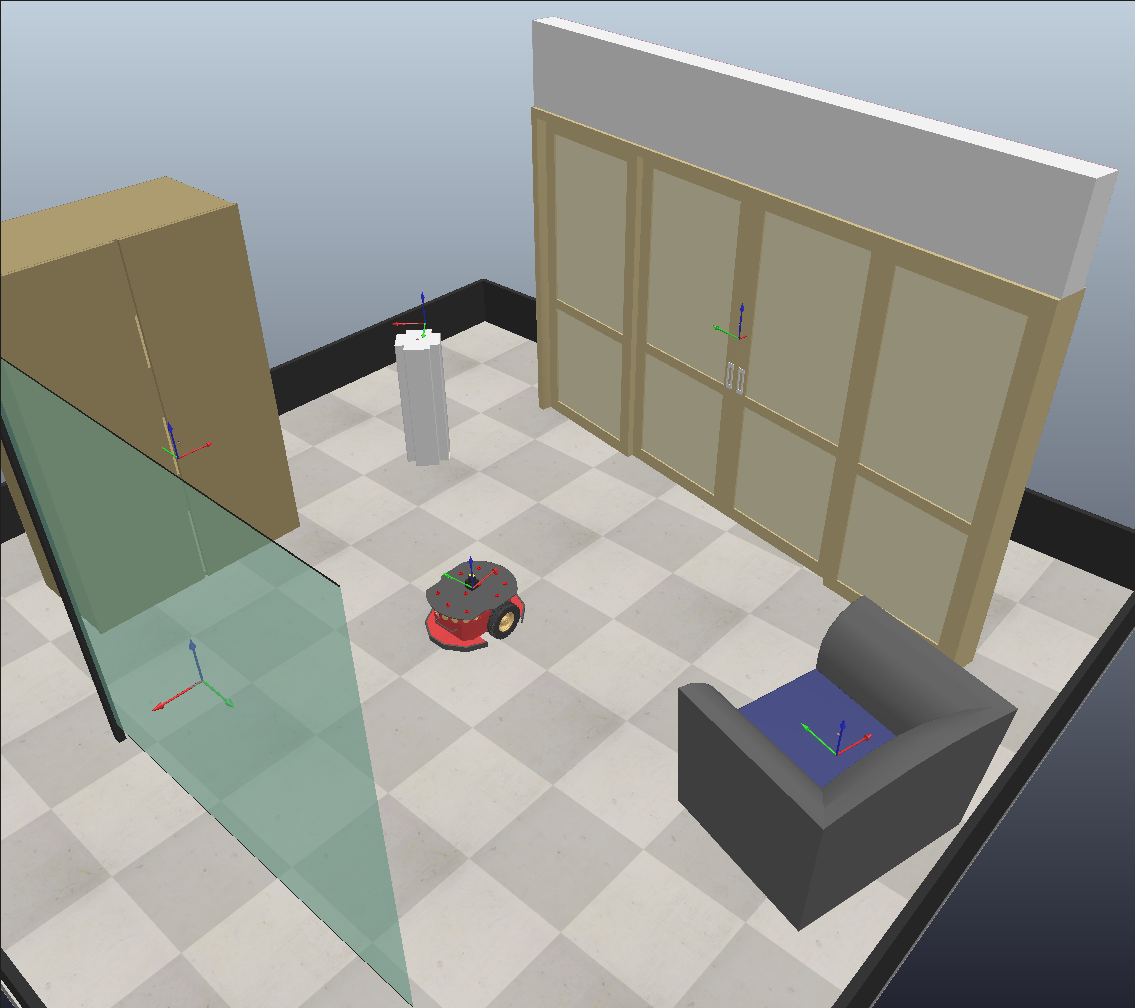
\includegraphics[width=\linewidth]{plots/q1.png}
  \caption{Q1 - Cena no CoppeliaSim com todos os objetos adicionados.}
\end{figure}

% ============================
\section*{Questão 2 \ \textnormal{[0,5 pts]}}
\textbf{Enunciado.}
Defina os sistemas de coordenadas de todos os itens (você deve adicioná-los na cena e afixar aos elementos para facilitar a visualização). Em seguida, você deverá representar os sistemas de coordenadas e as transformações entre eles (não precisa ser todos para todos) utilizando um diagrama, similar à figura abaixo (pode ser uma versão mais simplificada).

\vspace{6pt}
\textbf{Resposta.}
Foram definidos referenciais locais (frames) para o robô e para cada um dos cinco elementos da cena, fixados aos objetos correspondentes para facilitar a visualização. O diagrama a seguir resume as relações entre o robô e cada um dos elementos na cena:
\begin{figure}[H]
  \centering
  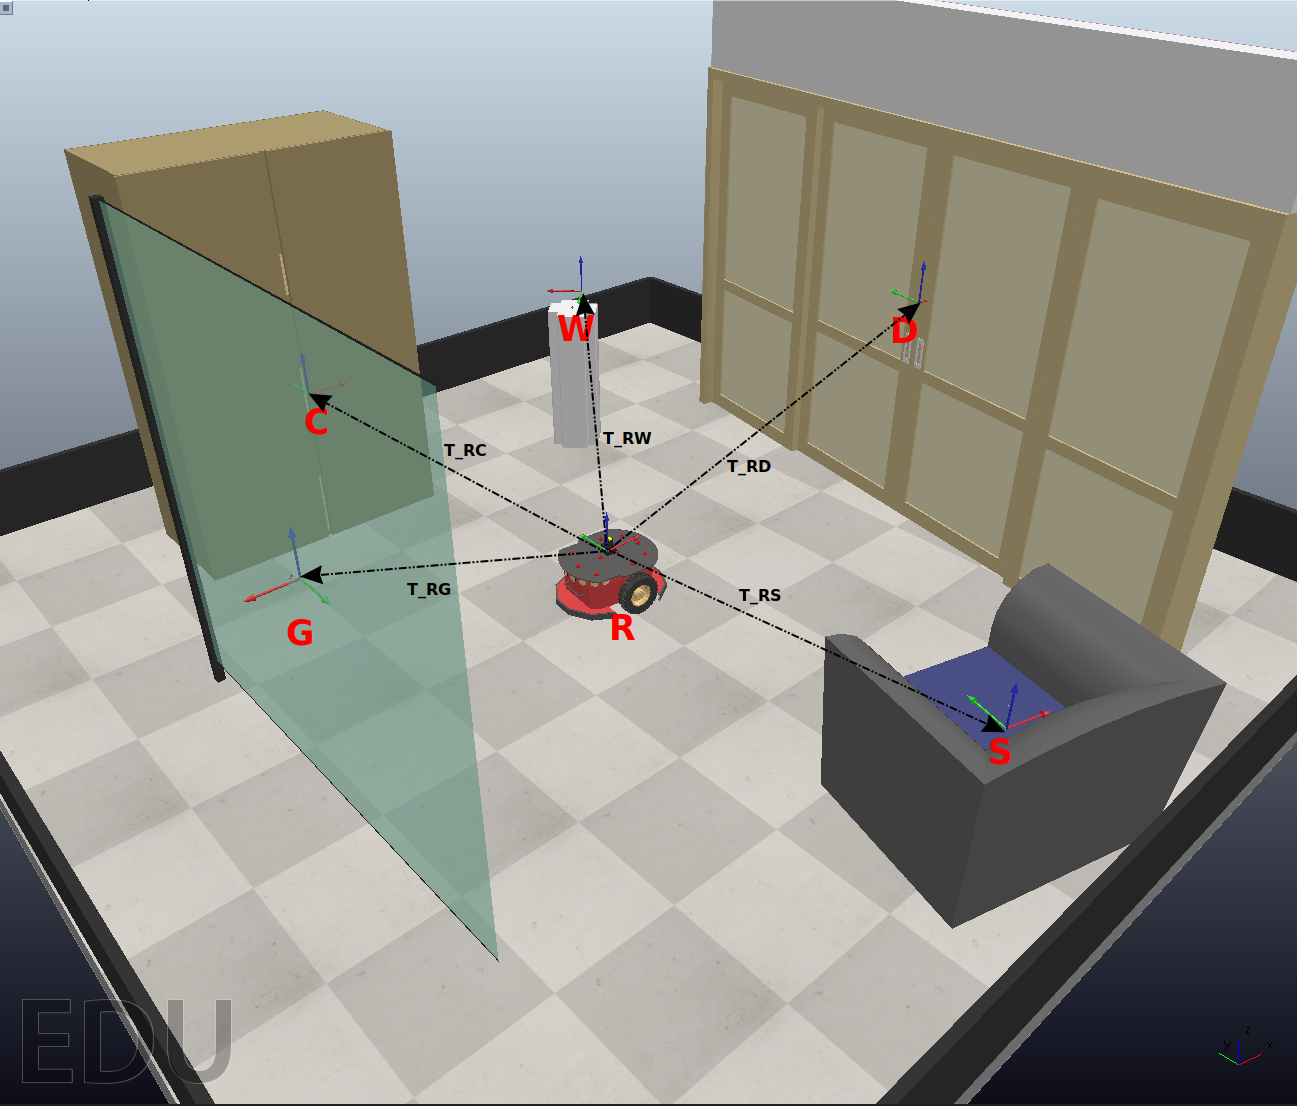
\includegraphics[width=\linewidth]{plots/q2.png}
  \caption{Q2 - Diagrama dos sistemas de coordenadas e transformações entre robô e objetos.}
\end{figure}

% ============================
\section*{Questão 3 \ \textnormal{[1,0 pt]}}
\textbf{Enunciado.}
Considerando que a configuração do robô no referencial global é conhecida e dada por \(q = [x, y, \theta]\), defina as matrizes de transformação homogêneas que representam as posições de todos os outros elementos da cena no referencial local do robô. Escreva um script que plota esses referenciais e os relacionamentos (vetor) entre eles (dica: use os códigos vistos em aula como base). Para os cálculos, as posições globais dos elementos podem ser recuperadas utilizando-se a RemoteAPI.

\vspace{6pt}
\textbf{Resposta.}
No plano (\(\SE(2)\)), a pose do robô no mundo é
\[
\mat{T'}^{W}_{R} =
\begin{bmatrix}
\cos\theta & -\sin\theta & x \\
\sin\theta & \phantom{-}\cos\theta & y \\
0 & 0 & 1
\end{bmatrix}.
\]
Em 3D, usando rotação em \(z\),
\[
\mat{T}^{W}_{R} =
\begin{bmatrix}
\cos\theta & -\sin\theta & 0 & x \\
\sin\theta & \phantom{-}\cos\theta & 0 & y \\
0 & 0 & 1 & 0 \\
0 & 0 & 0 & 1
\end{bmatrix}.
\]
Dado um objeto \(O_i\) com pose global \(\mat{T}^{W}_{O_i}\), a pose desse objeto no referencial do robô é
\[
\mat{T}^{R}_{O_i} = \big(\mat{T}^{W}_{R}\big)^{-1}\, \mat{T}^{W}_{O_i}.
\]
Os vetores ligando a origem do robô aos objetos (\emph{e.g.}, do \(R\) ao \(O_i\)) são extraídos como \(\vect{p}^{R}_{O_i}\) a partir do termo de translação de \(\mat{T}^{R}_{O_i}\).
O script produz os referenciais e os vetores de relacionamento e gera o seguinte plot:
\begin{figure}[H]
  \centering
  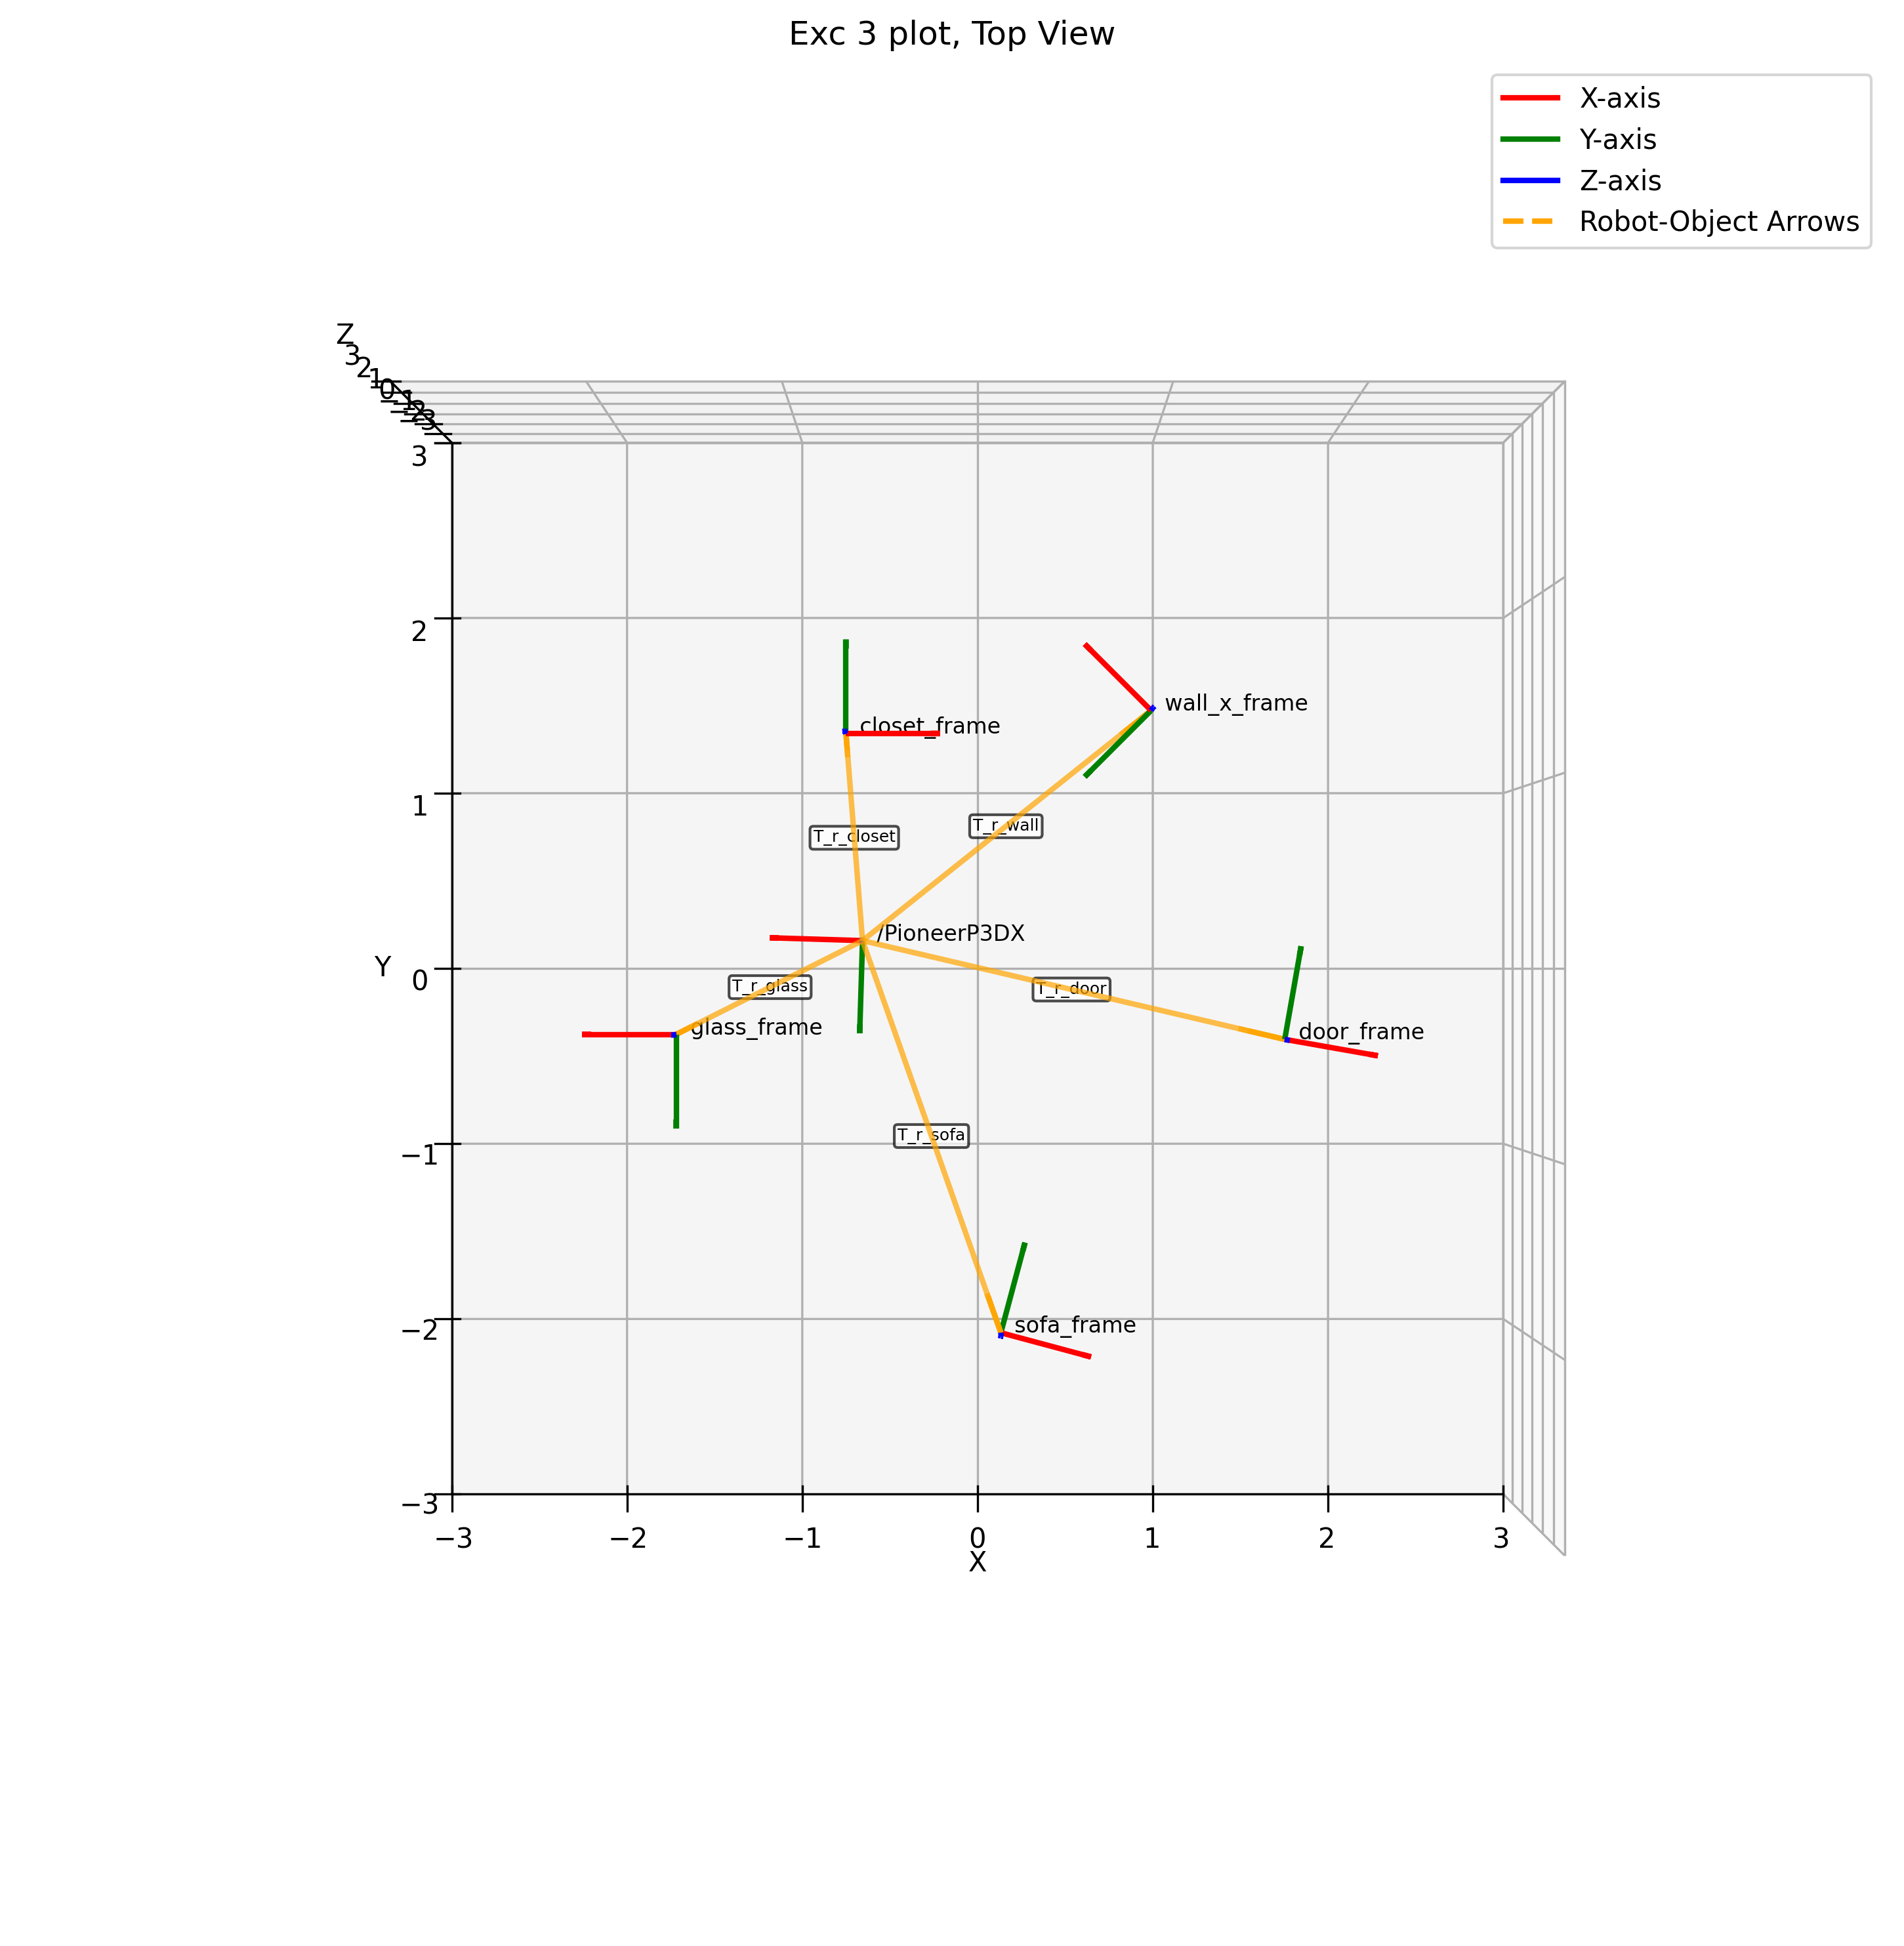
\includegraphics[width=\linewidth]{plots/q3.png}
  \caption{Q3 - Referenciais e vetores \(R \rightarrow O_i\) (cena original).}
\end{figure}

Considerando \textbf{G, S, D, X, C} como os frames dos objetos 'Glass', 'Sofa', 'Door, 'X Wall' e 'Closet' respectivamente, e \textbf{W} o frame global, temos as transformadas mostradas na tabela \ref{tab:q3}.

\setlength{\arraycolsep}{4pt}
\noindent
\begin{tcolorbox}[enhanced,attach boxed title to top center={yshift=-3mm,yshifttext=-1mm}, colback=blue!5!white, colframe=blue!75!black, colbacktitle=blue!40!white, title=Homogeneous transforms for robot initial pose,fonttitle=\bfseries, boxed title style={size=small,colframe=blue!50!black} ]
  \label{tab:q3}
    \begin{minipage}[t]{0.49\linewidth}
    \small
    \[
    \mat{T}^{W}_{R} =
    \begin{bmatrix}
     1.00 & 0.00 & 0.00 & 0.00 \\
     0.00 & 1.00 & 0.00 & 0.00 \\
     0.00 &  0.00 & 1.00 & 0.14 \\
     0.00 &  0.00 & 0.00 & 1.00
    \end{bmatrix}
    \]
    \vspace{8pt}
    \[
    \mat{T}^{R}_{G} =
    \begin{bmatrix}
     0.99 & -0.14 &  0.00 &  0.68 \\
     0.14 &  0.99 &  0.00 &  0.56 \\
     0.00 &  0.00 &  1.00 &  0.86 \\
     0.00 &  0.00 &  0.00 &  1.00
    \end{bmatrix}
    \]
    \vspace{8pt}
    \[
    \mat{T}^{R}_{D} =
    \begin{bmatrix}
     -1.00 & -0.04 &  0.00 & -2.52 \\
      0.04 & -1.00 &  0.00 &  0.14 \\
      0.00 &  0.00 &  1.00 &  1.07 \\
      0.00 &  0.00 &  0.00 &  1.00
    \end{bmatrix}
    \]
    \end{minipage}\hfill
    \begin{minipage}[t]{0.49\linewidth}
    \small
    \[
    \mat{T}^{R}_{C} =
    \begin{bmatrix}
     -0.99 &  0.14 &  0.00 &  0.01 \\
     -0.14 & -0.99 &  0.00 & -1.15 \\
      0.00 &  0.00 &  1.00 &  0.76 \\
      0.00 &  0.00 &  0.00 &  1.00
    \end{bmatrix}
    \]
    \vspace{8pt}
    \[
    \mat{T}^{R}_{S} =
    \begin{bmatrix}
     -0.99 & -0.12 &  0.00 & -1.25 \\
      0.12 & -0.99 &  0.00 &  1.91 \\
      0.00 &  0.00 &  1.00 &  0.36 \\
      0.00 &  0.00 &  0.00 &  1.00
    \end{bmatrix}
    \]
    \vspace{8pt}
    \[
    \mat{T}^{R}_{X} =
    \begin{bmatrix}
      0.80 &  0.60 &  0.00 & -1.59 \\
     -0.60 &  0.80 &  0.00 & -1.50 \\
      0.00 &  0.00 &  1.00 &  0.67 \\
      0.00 &  0.00 &  0.00 &  1.00
    \end{bmatrix}
    \]
    \end{minipage}
\end{tcolorbox}
% ============================
\section*{Questão 4 \ \textnormal{[0,5 pts]}}
\textbf{Enunciado.}
Coloque o robô em outras três posições diferentes da cena e faça os respectivos plots (referenciais e relacionamentos), verificando que a implementação funciona para diferentes casos. Lembre-se de também variar a orientação do robô em relação aos elementos, por exemplo, colocando ele de frente, de lado e de costas.

\vspace{6pt}
\textbf{Resposta.}
Foram testadas três poses adicionais do robô, variando posição e orientação. Em cada caso, computou-se \(\mat{T}^{R}_{O_i}\) via \(\big(\mat{T}^{W}_{R}\big)^{-1}\mat{T}^{W}_{O_i}\) e atualizou-se o diagrama de referenciais e vetores.
\begin{figure}[H]
  \centering
  \begin{subfigure}[t]{0.49\linewidth}
    \centering
    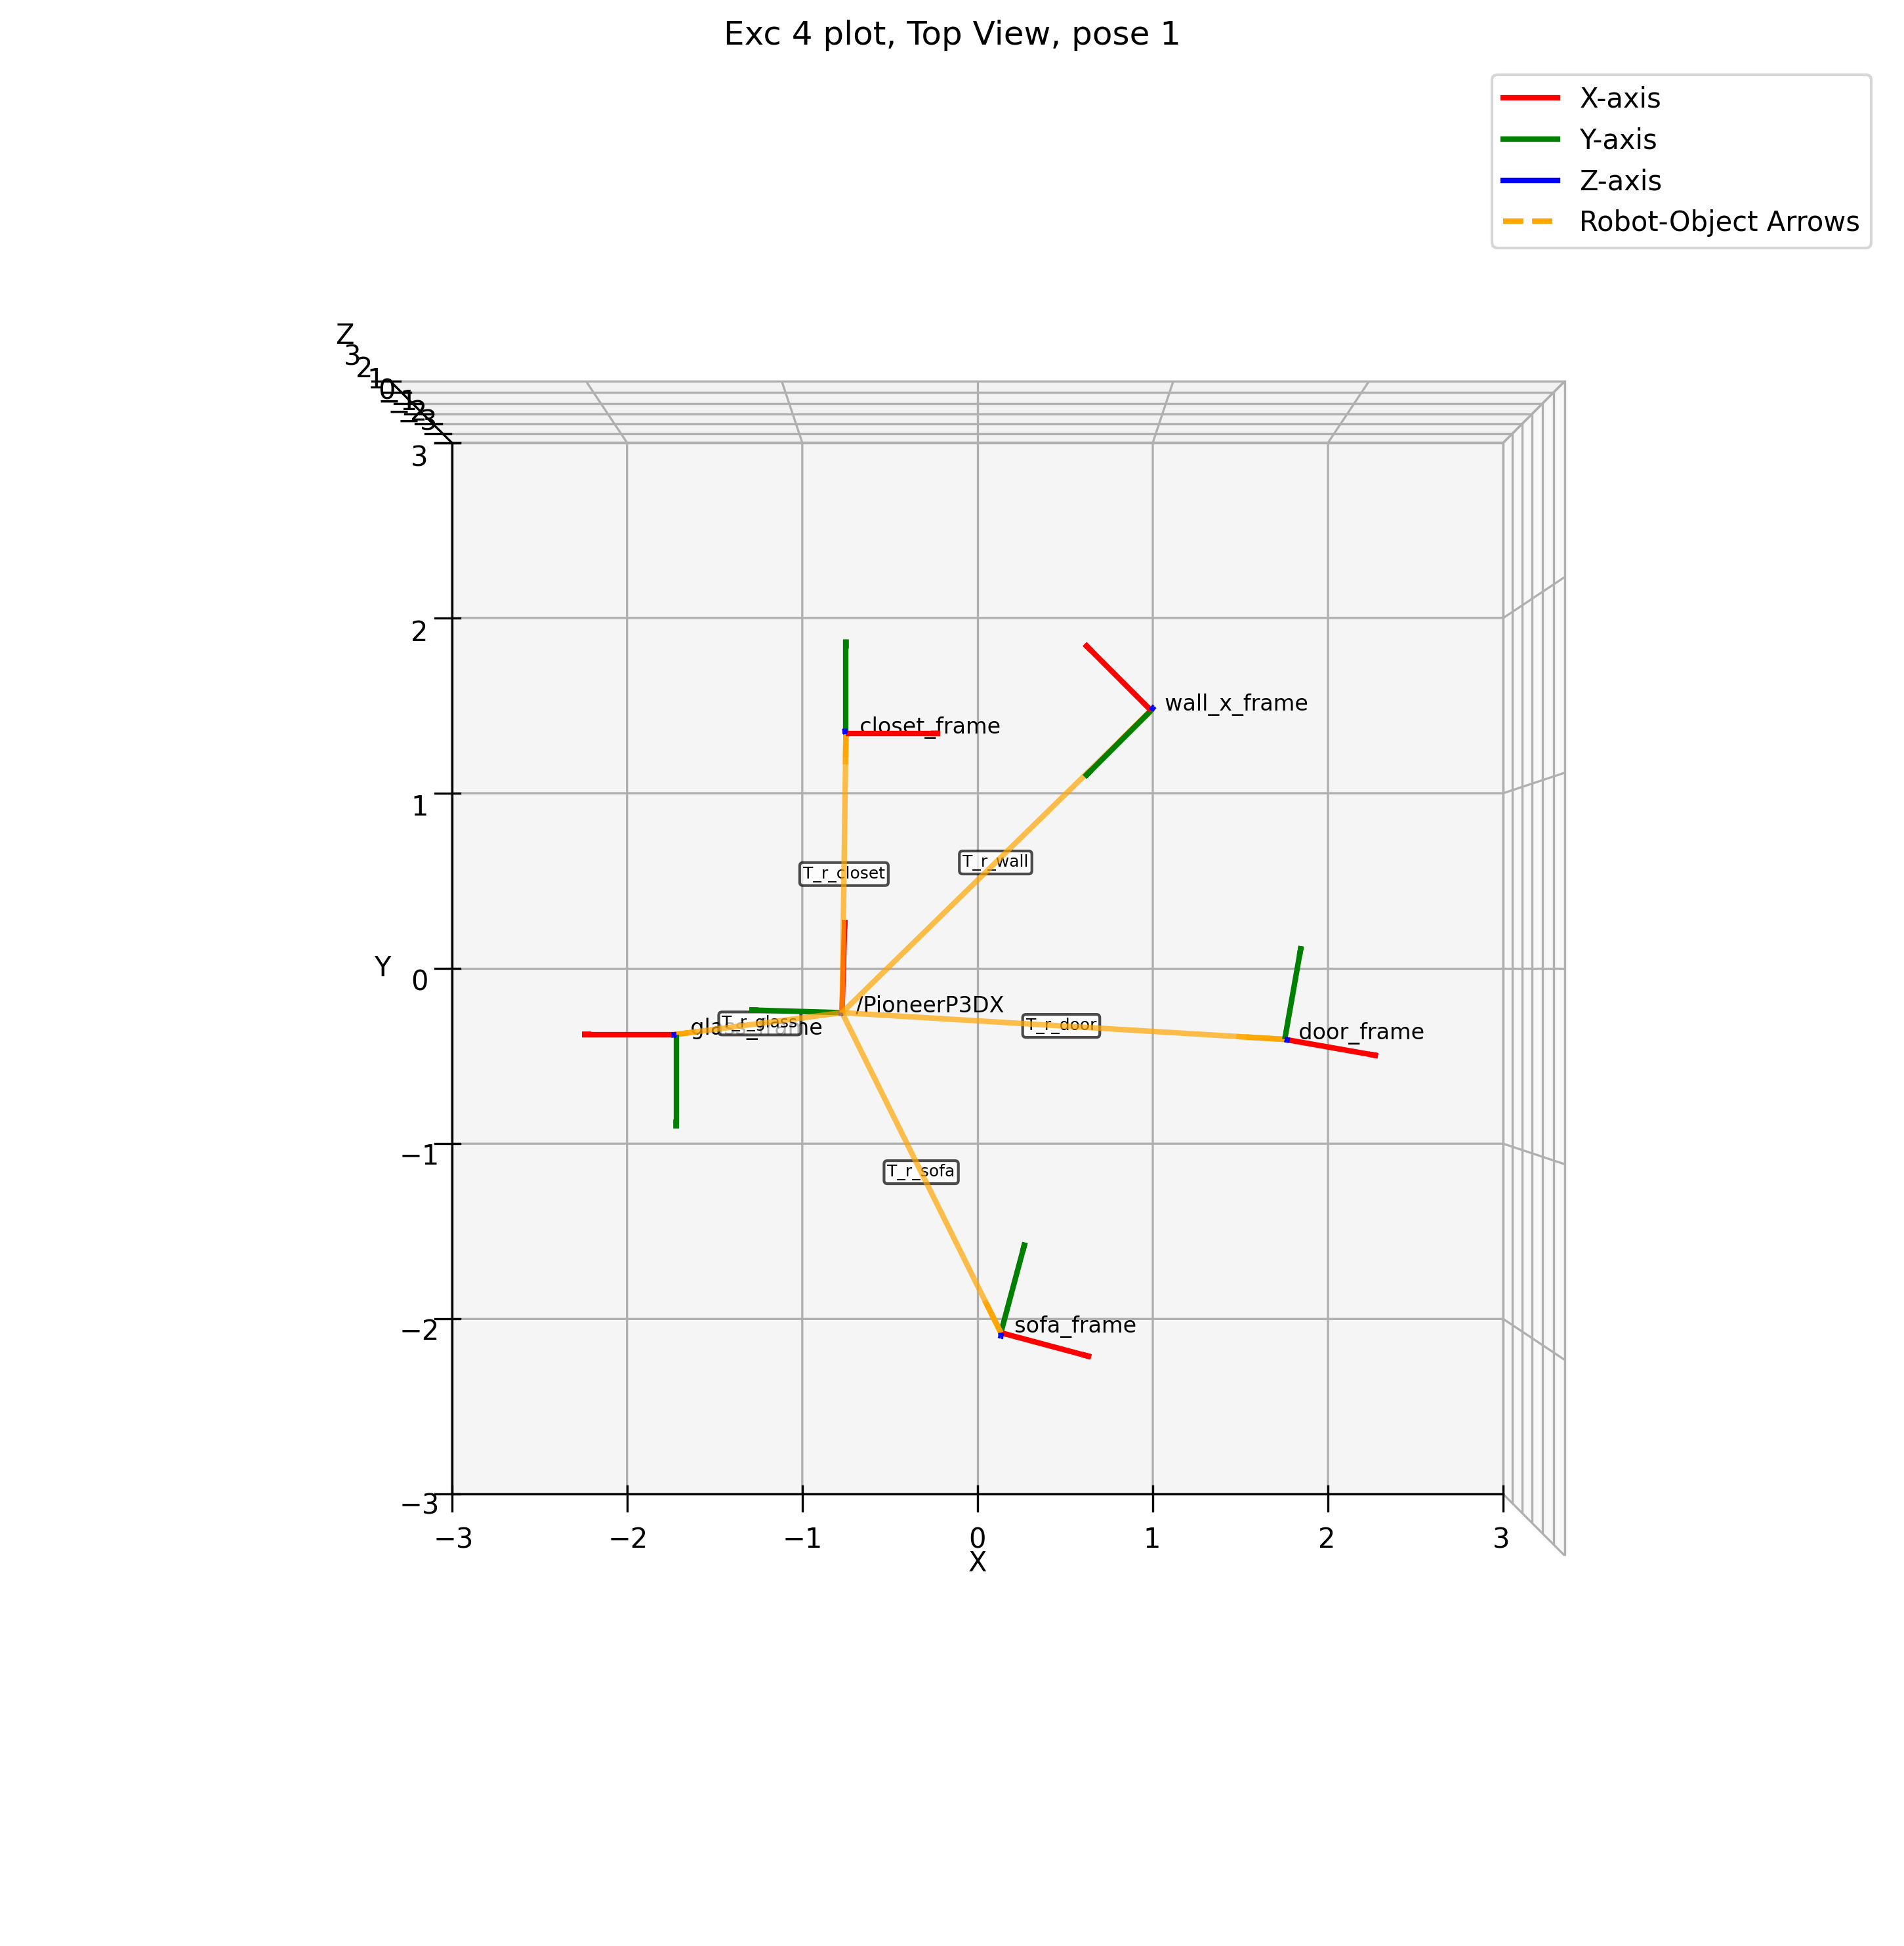
\includegraphics[width=\linewidth]{plots/q4_top_view_plot_1.png}
    \caption{Vista superior.}
    \label{fig:q4:a}
  \end{subfigure}\hfill
  \begin{subfigure}[t]{0.49\linewidth}
    \centering
    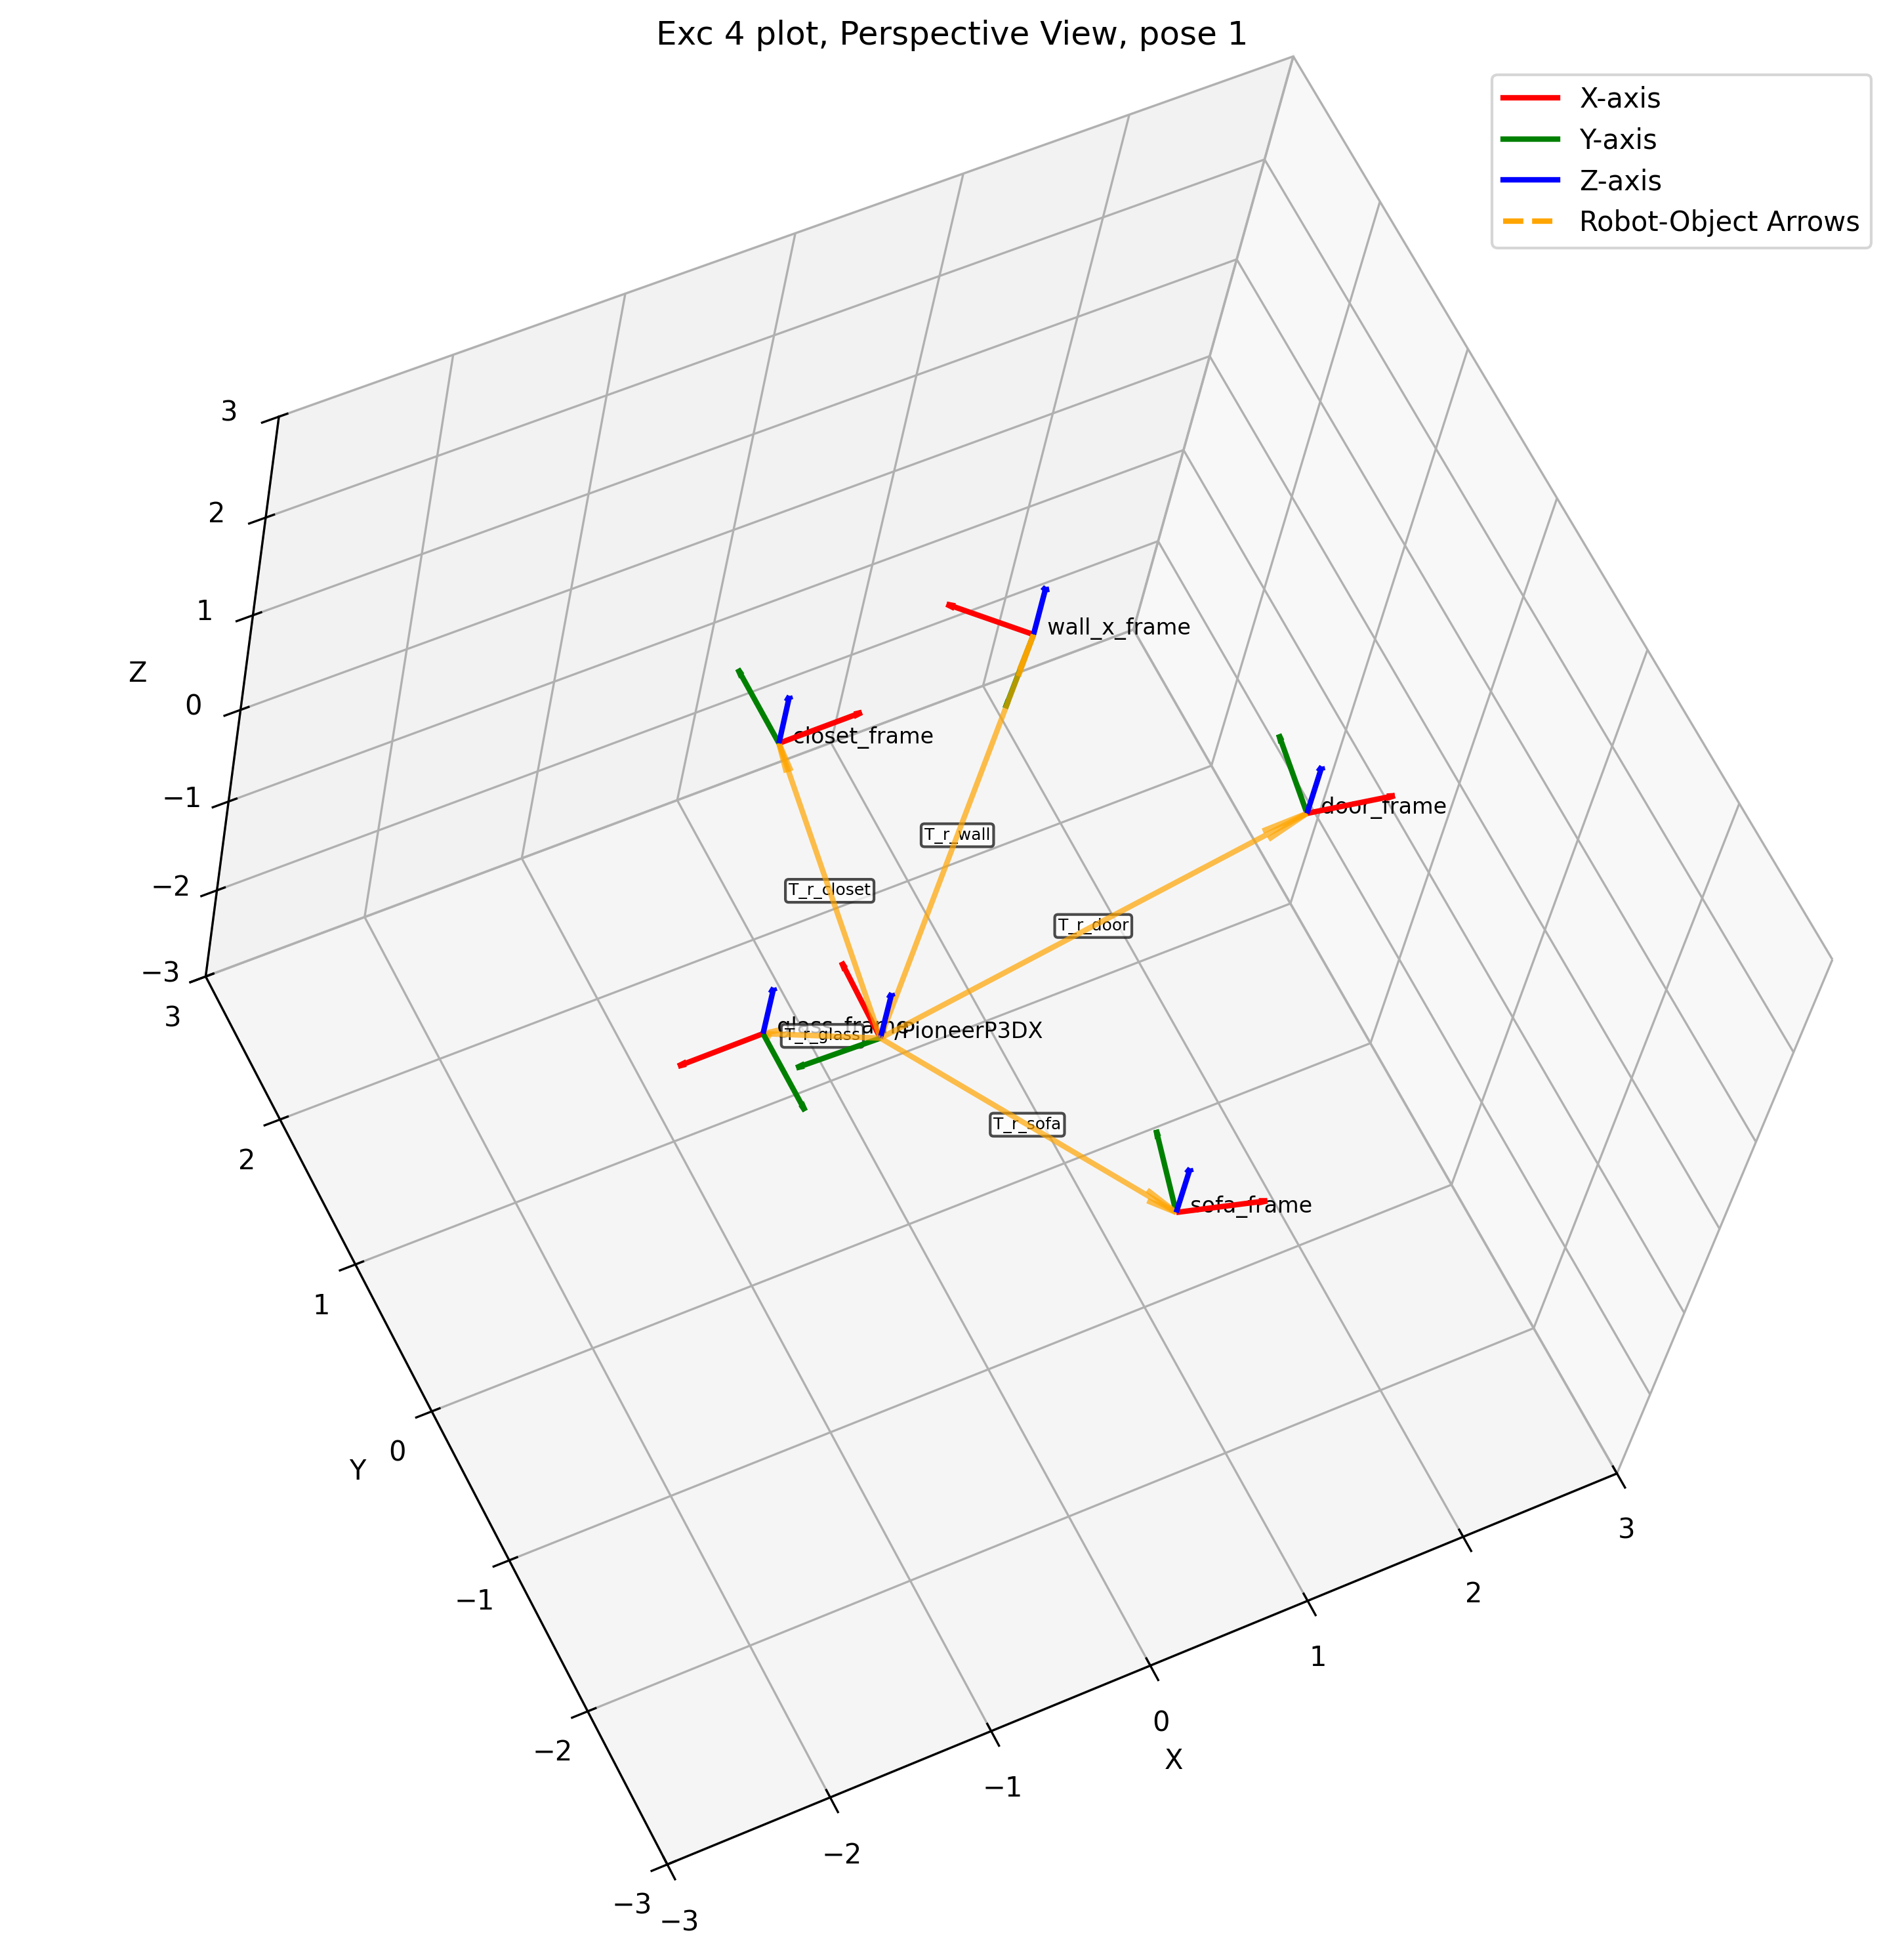
\includegraphics[width=\linewidth]{plots/q4_perspective_plot_1.png}
    \caption{Vista em perspectiva.}
    \label{fig:q4:b}
  \end{subfigure}
  \caption{Q4 - Resultados para pose 1 do robô.}
  \label{fig:q4}
\end{figure}

\noindent
\begin{tcolorbox}[enhanced,attach boxed title to top center={yshift=-3mm,yshifttext=-1mm}, colback=blue!5!white, colframe=blue!75!black, colbacktitle=blue!40!white, title=Homogeneous transforms for Random Pose 1,fonttitle=\bfseries, boxed title style={size=small,colframe=blue!50!black} ]

    \label{tab:q4_1}
    \begin{minipage}[t]{0.49\linewidth}
    \small
    \[
    \mat{T}^{W}_{R} =
    \begin{bmatrix}
     -0.45 & -0.89 & 0.00 & 0.78 \\
     0.89 &  -0.45 & 0.00 & 0.00 \\
     0.00 &  0.00 & 1.00 & 0.14 \\
     0.00 &  0.00 & 0.00 & 1.00
    \end{bmatrix}
    \]
    \vspace{8pt}
    \[
    \mat{T}^{R}_{G} =
    \begin{bmatrix}
     0.45 & -0.89 & 0.00 & 0.77 \\
     0.89 &  0.45 & 0.00 & 2.28 \\
     0.00 &  0.00 & 1.00 & 0.86 \\
     0.00 &  0.00 & 0.00 & 1.00
    \end{bmatrix}
    \]
    \vspace{8pt}
    \[
    \mat{T}^{R}_{D} =
    \begin{bmatrix}
     -0.60 &  0.80 & 0.00 & -0.72 \\
     -0.80 & -0.60 & 0.00 & -0.58 \\
      0.00 &  0.00 & 1.00 &  1.06 \\
      0.00 &  0.00 & 0.00 &  1.00
    \end{bmatrix}
    \]
    \end{minipage}\hfill
    \begin{minipage}[t]{0.49\linewidth}
    \small
    \[
    \mat{T}^{R}_{C} =
    \begin{bmatrix}
     -0.45 &  0.89 & 0.00 & 1.79 \\
     -0.89 & -0.45 & 0.00 & 0.75 \\
      0.00 &  0.00 & 1.00 & 0.76 \\
      0.00 &  0.00 & 0.00 & 1.00
    \end{bmatrix}
    \]
    \vspace{8pt}
    \[
    \mat{T}^{R}_{S} =
    \begin{bmatrix}
     -0.67 &  0.74 & 0.00 & -1.44 \\
     -0.74 & -0.67 & 0.00 &  1.47 \\
      0.00 &  0.00 & 1.00 &  0.36 \\
      0.00 &  0.00 & 0.00 &  1.00
    \end{bmatrix}
    \]
    \vspace{8pt}
    \[
    \mat{T}^{R}_{X} =
    \begin{bmatrix}
     0.95 & -0.31 & 0.00 &  1.16 \\
     0.31 &  0.95 & 0.00 & -0.75 \\
     0.00 &  0.00 & 1.00 &  0.66 \\
     0.00 &  0.00 & 0.00 &  1.00
    \end{bmatrix}
    \]
    \end{minipage}
\end{tcolorbox}

\begin{figure}[H]
  \centering
  \begin{subfigure}[t]{0.49\linewidth}
    \centering
    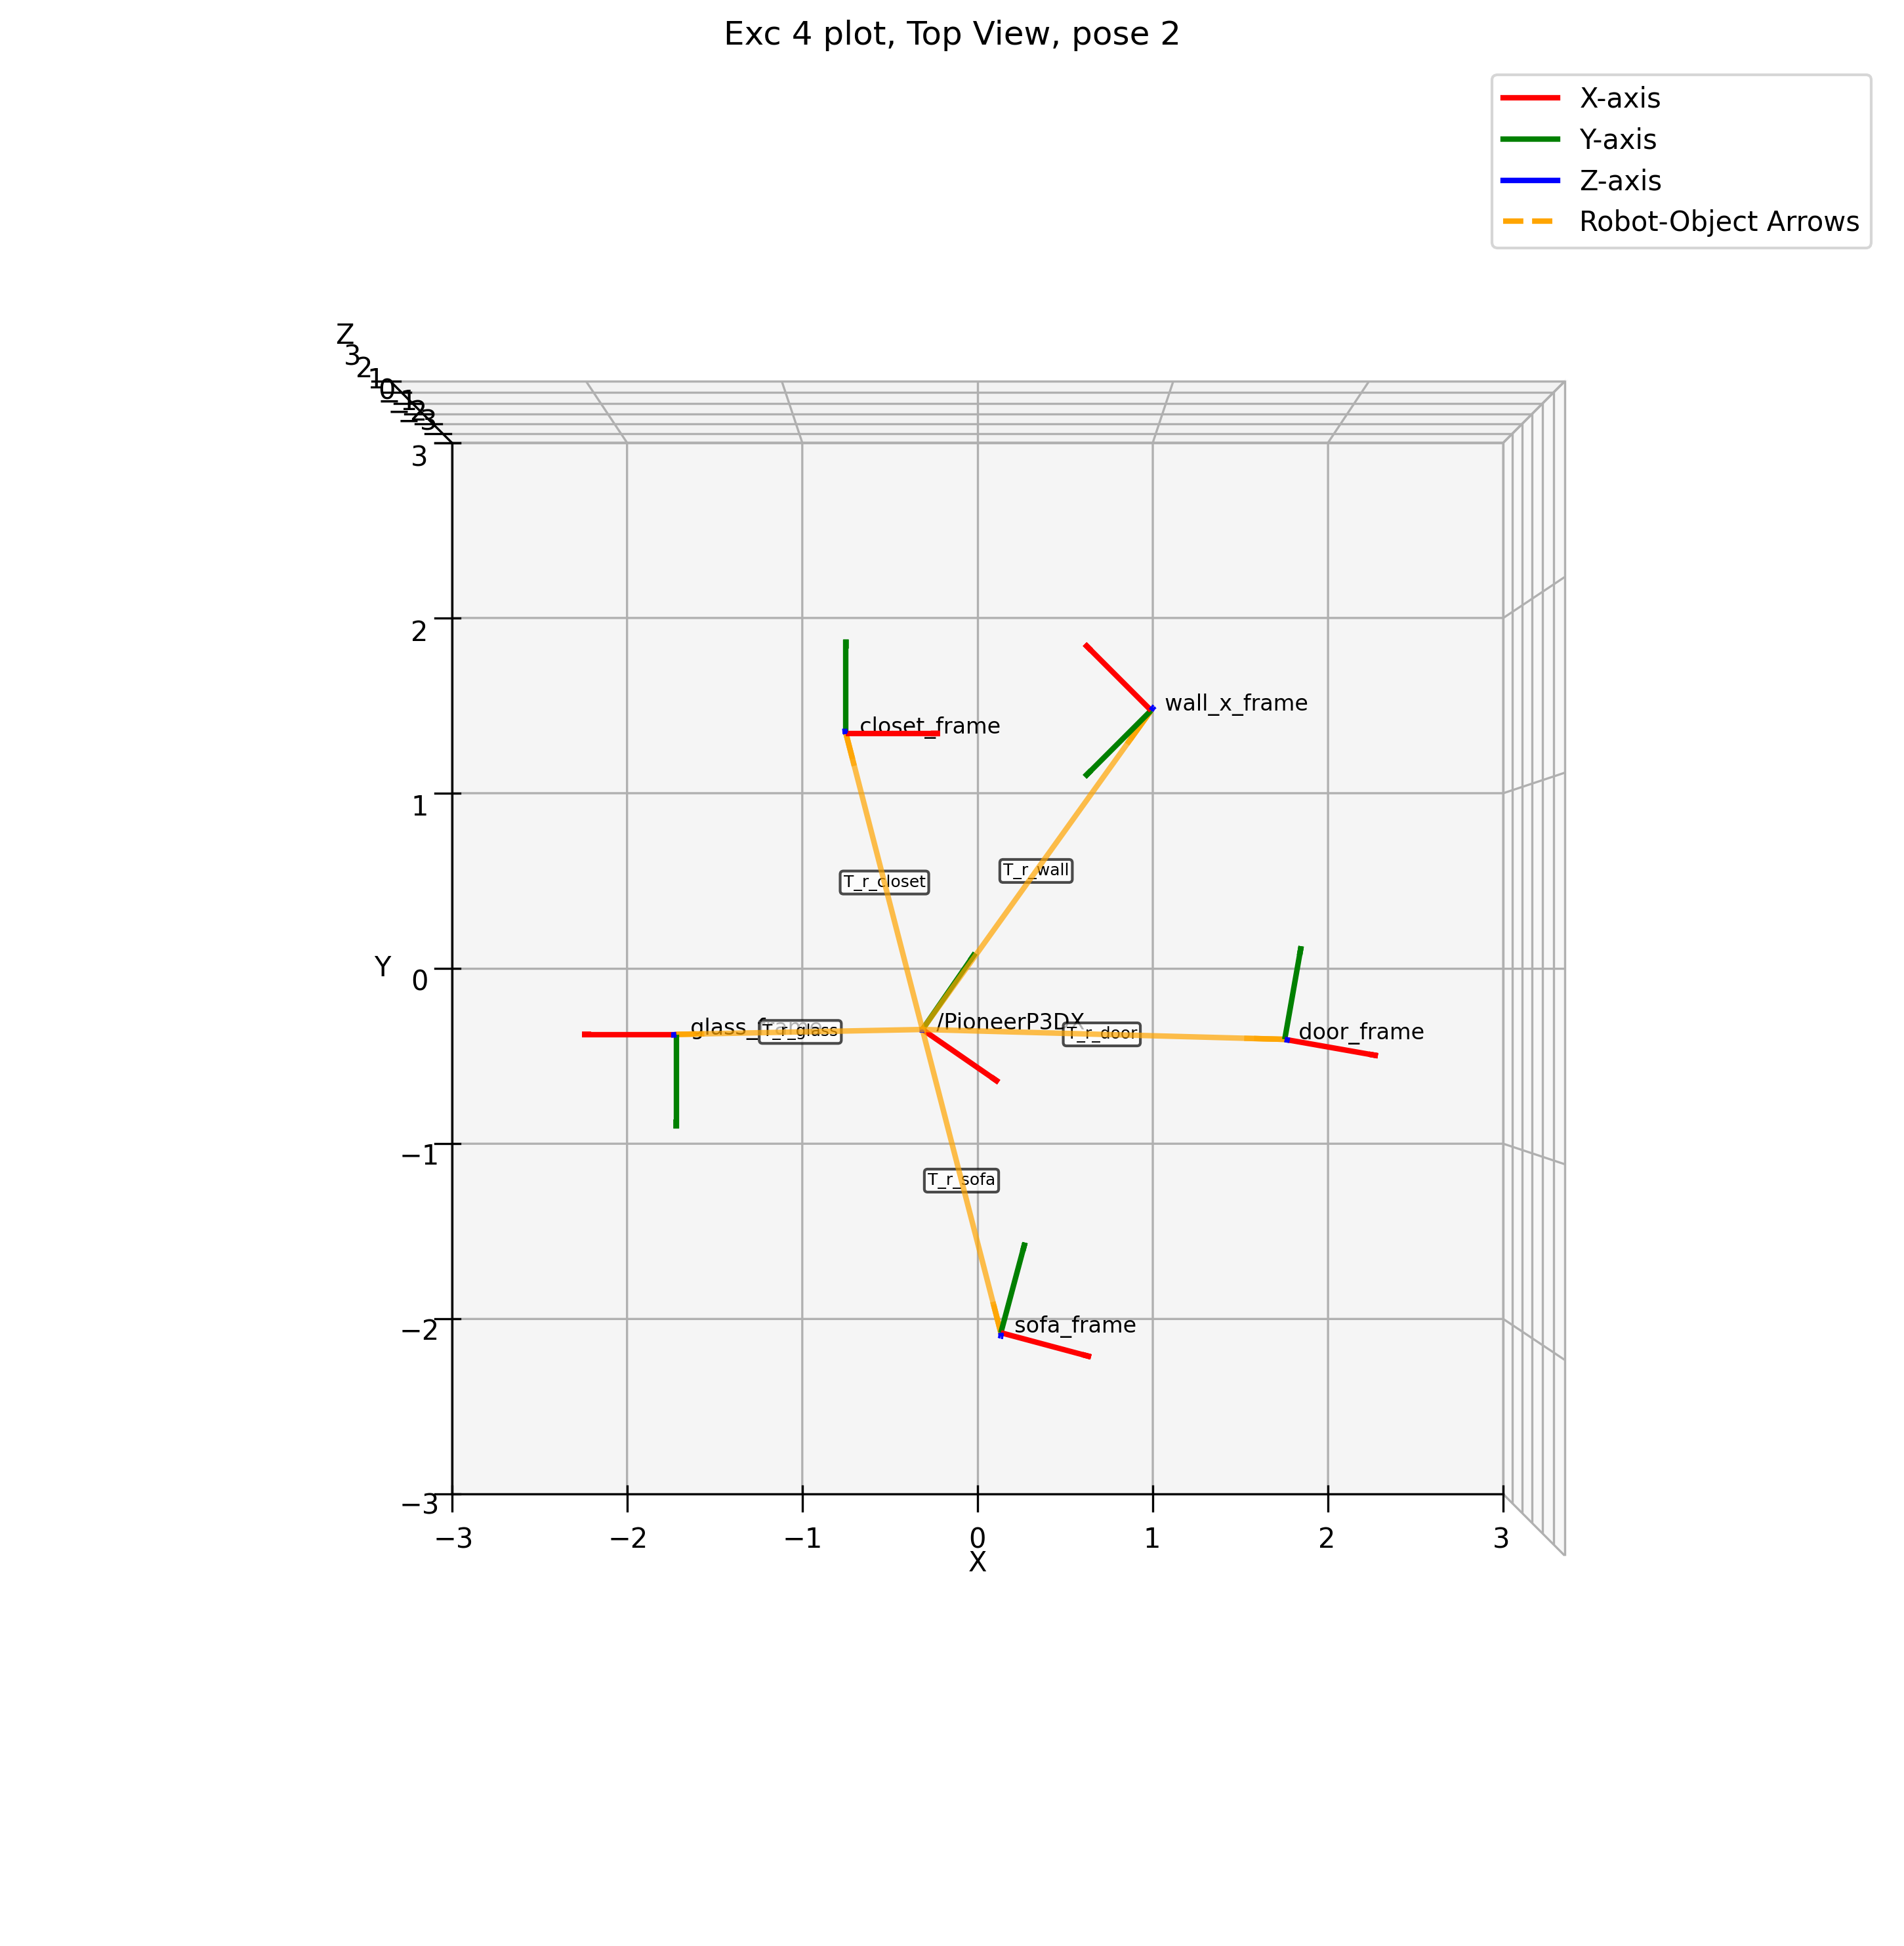
\includegraphics[width=\linewidth]{plots/q4_top_view_plot_2.png}
    \caption{Vista superior.}
    \label{fig:q4:a}
  \end{subfigure}\hfill
  \begin{subfigure}[t]{0.49\linewidth}
    \centering
    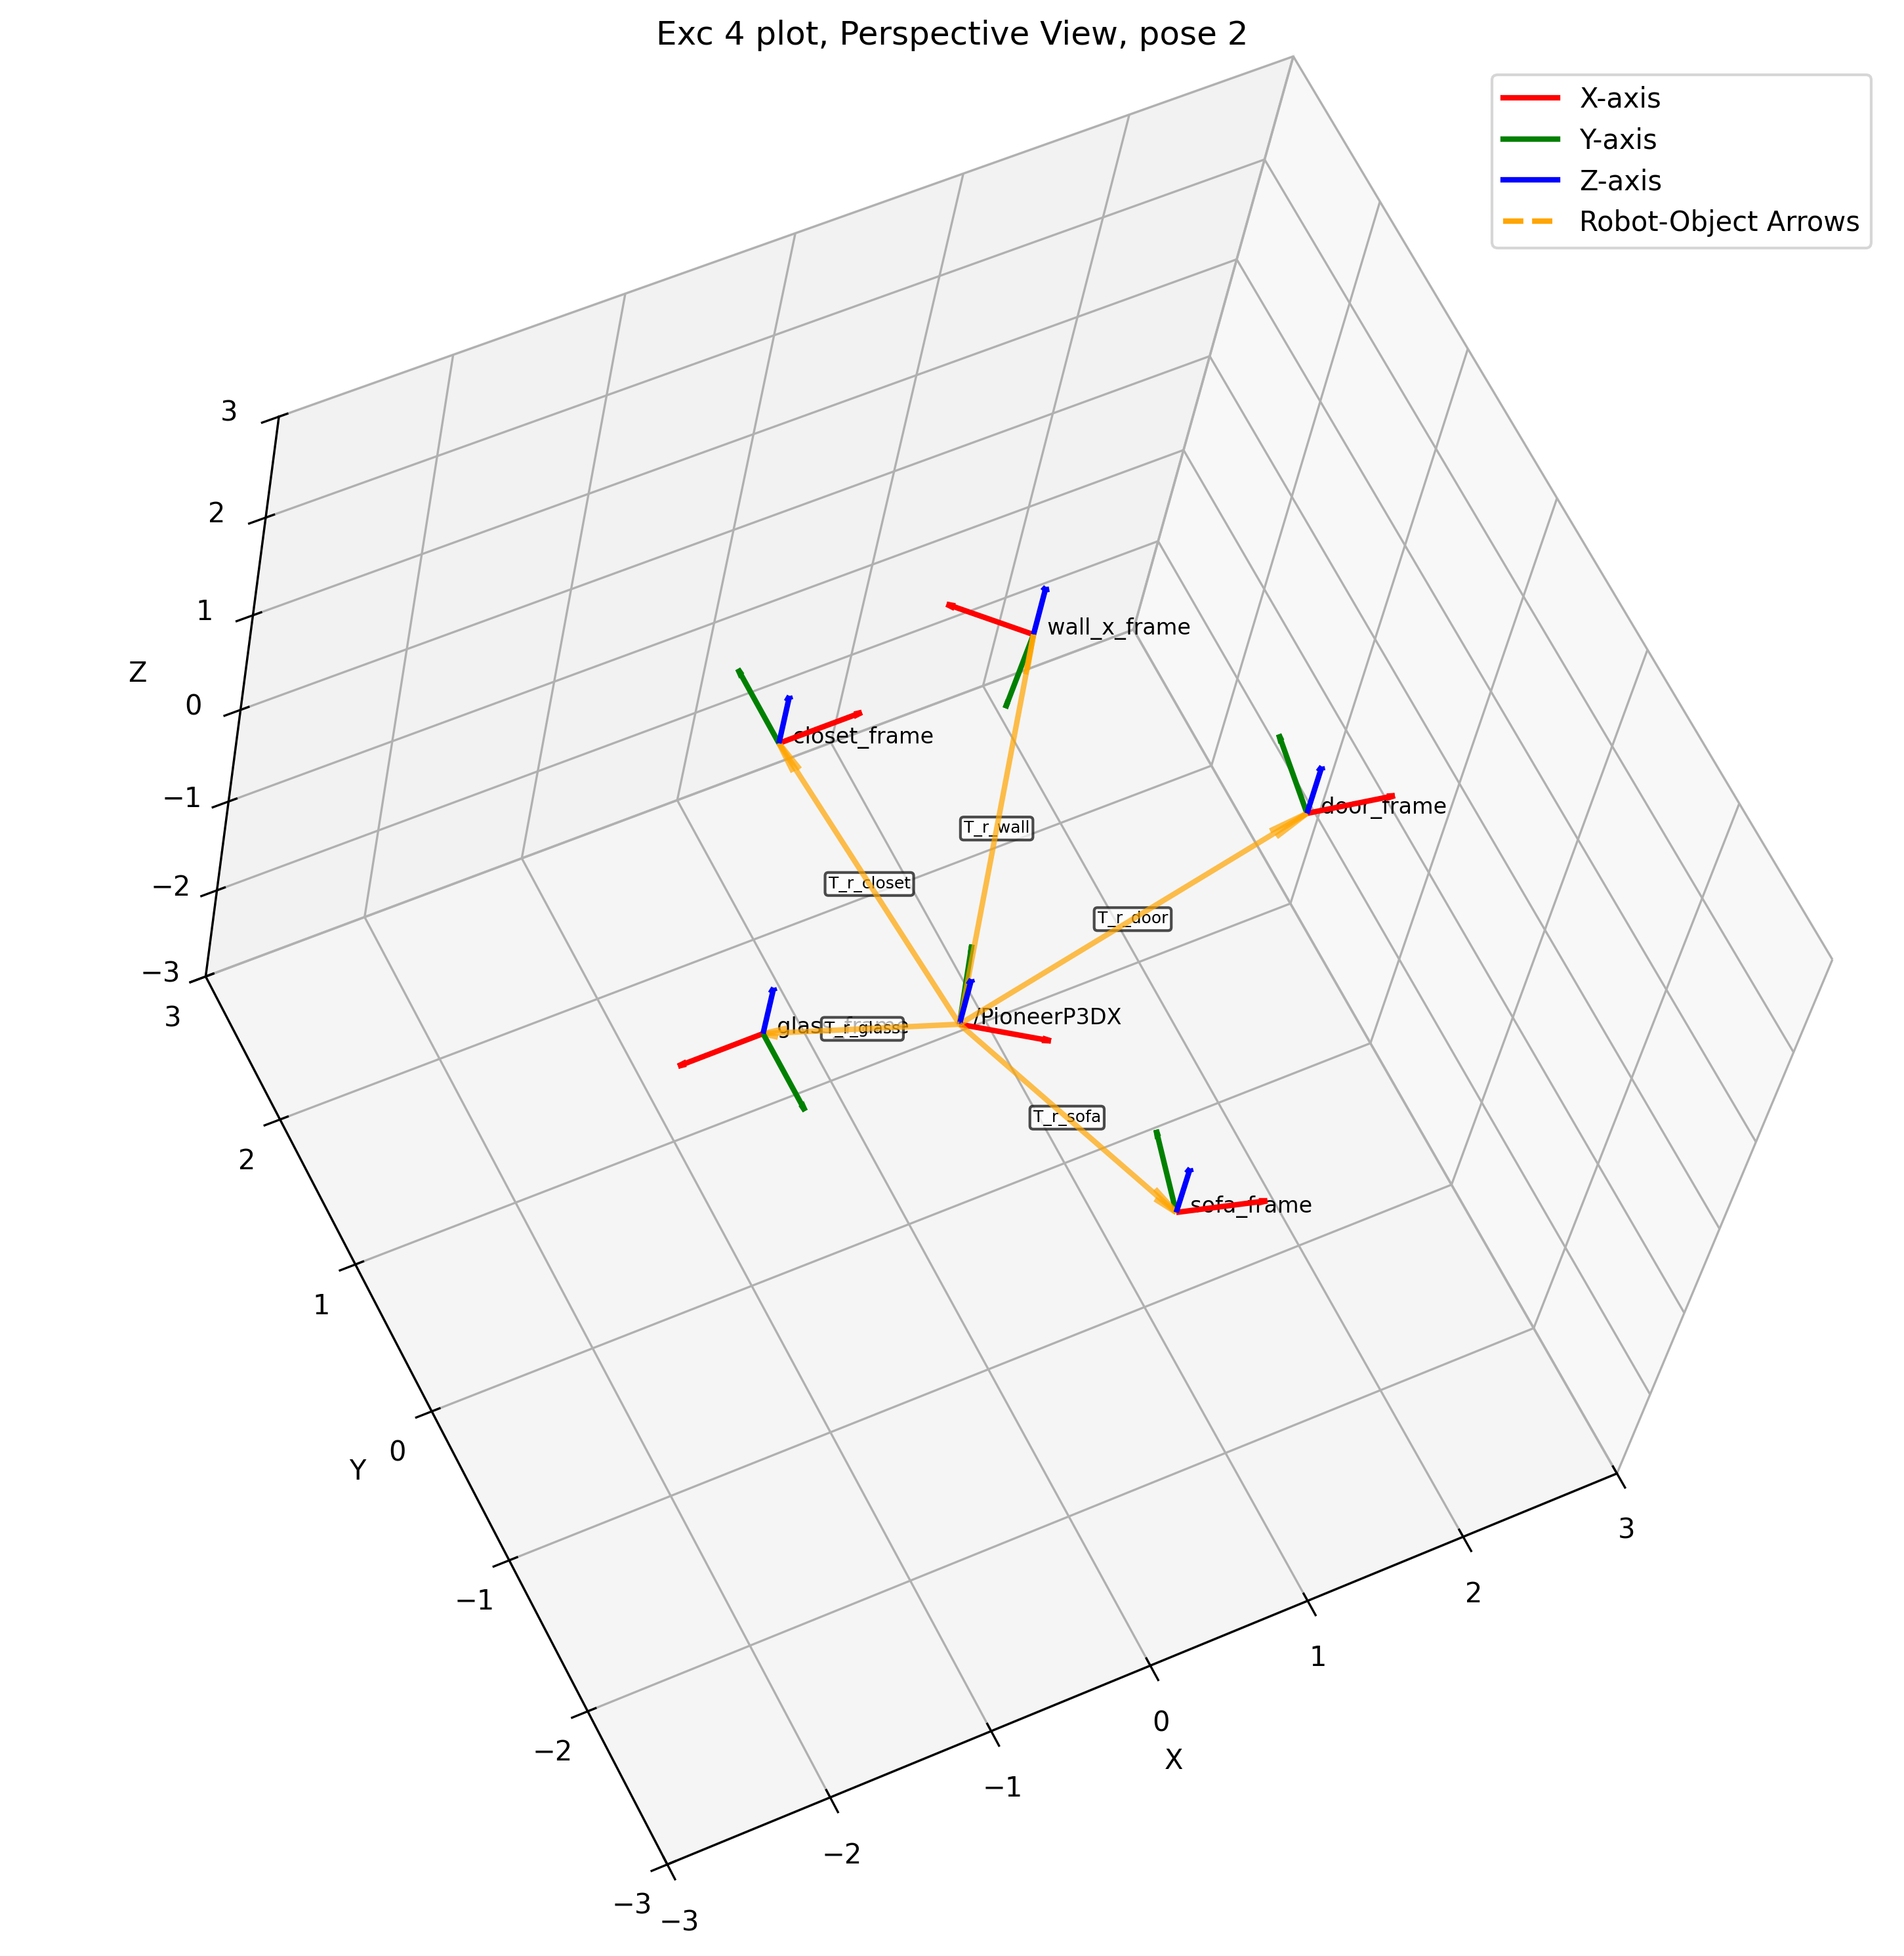
\includegraphics[width=\linewidth]{plots/q4_perspective_plot_2.png}
    \caption{Vista em perspectiva.}
    \label{fig:q4:b}
  \end{subfigure}
  \caption{Q4 - Resultados para pose 2 do robô.}
  \label{fig:q4}
\end{figure}

\noindent
\begin{tcolorbox}[enhanced,attach boxed title to top center={yshift=-3mm,yshifttext=-1mm}, colback=blue!5!white, colframe=blue!75!black, colbacktitle=blue!40!white, title=Homogeneous transforms for Random Pose 2,fonttitle=\bfseries, boxed title style={size=small,colframe=blue!50!black} ]
    \label{tab:q4_2}
    \begin{minipage}[t]{0.49\linewidth}
    \small
    \[
    \mat{T}^{W}_{R} =
    \begin{bmatrix}
     0.97 & 0.24 & 0.00 & 0.05 \\
     -0.24 & 0.97 & 0.00 & 0.21 \\
     0.00 &  0.00 & 1.00 & 0.14 \\
     0.00 &  0.00 & 0.00 & 1.00
    \end{bmatrix}
    \]
    \vspace{8pt}
    \[
    \mat{T}^{R}_{G} =
    \begin{bmatrix}
     -0.97 &  0.24 & 0.00 & -1.47 \\
     -0.24 & -0.97 & 0.00 & -0.94 \\
      0.00 &  0.00 & 1.00 &  0.86 \\
      0.00 &  0.00 & 0.00 &  1.00
    \end{bmatrix}
    \]
    \vspace{8pt}
    \[
    \mat{T}^{R}_{D} =
    \begin{bmatrix}
     1.00 & -0.07 & 0.00 &  1.66 \\
     0.07 &  1.00 & 0.00 & -0.19 \\
     0.00 &  0.00 & 1.00 &  1.06 \\
     0.00 &  0.00 & 0.00 &  1.00
    \end{bmatrix}
    \]
    \end{minipage}\hfill
    \begin{minipage}[t]{0.49\linewidth}
    \small
    \[
    \mat{T}^{R}_{C} =
    \begin{bmatrix}
     0.97 & -0.24 & 0.00 & -0.98 \\
     0.24 &  0.97 & 0.00 &  0.83 \\
     0.00 &  0.00 & 1.00 &  0.76 \\
     0.00 &  0.00 & 0.00 &  1.00
    \end{bmatrix}
    \]
    \vspace{8pt}
    \[
    \mat{T}^{R}_{S} =
    \begin{bmatrix}
      1.00 &  0.02 & 0.00 &  0.59 \\
     -0.02 &  1.00 & 0.00 & -2.08 \\
      0.00 &  0.00 & 1.00 &  0.36 \\
      0.00 &  0.00 & 0.00 &  1.00
    \end{bmatrix}
    \]
    \vspace{8pt}
    \[
    \mat{T}^{R}_{X} =
    \begin{bmatrix}
     -0.86 & -0.51 & 0.00 &  0.56 \\
      0.51 & -0.86 & 0.00 &  1.34 \\
      0.00 &  0.00 & 1.00 &  0.66 \\
      0.00 &  0.00 & 0.00 &  1.00
    \end{bmatrix}
    \]
    \end{minipage}
\end{tcolorbox}

\begin{figure}[H]
  \centering
  \begin{subfigure}[t]{0.49\linewidth}
    \centering
    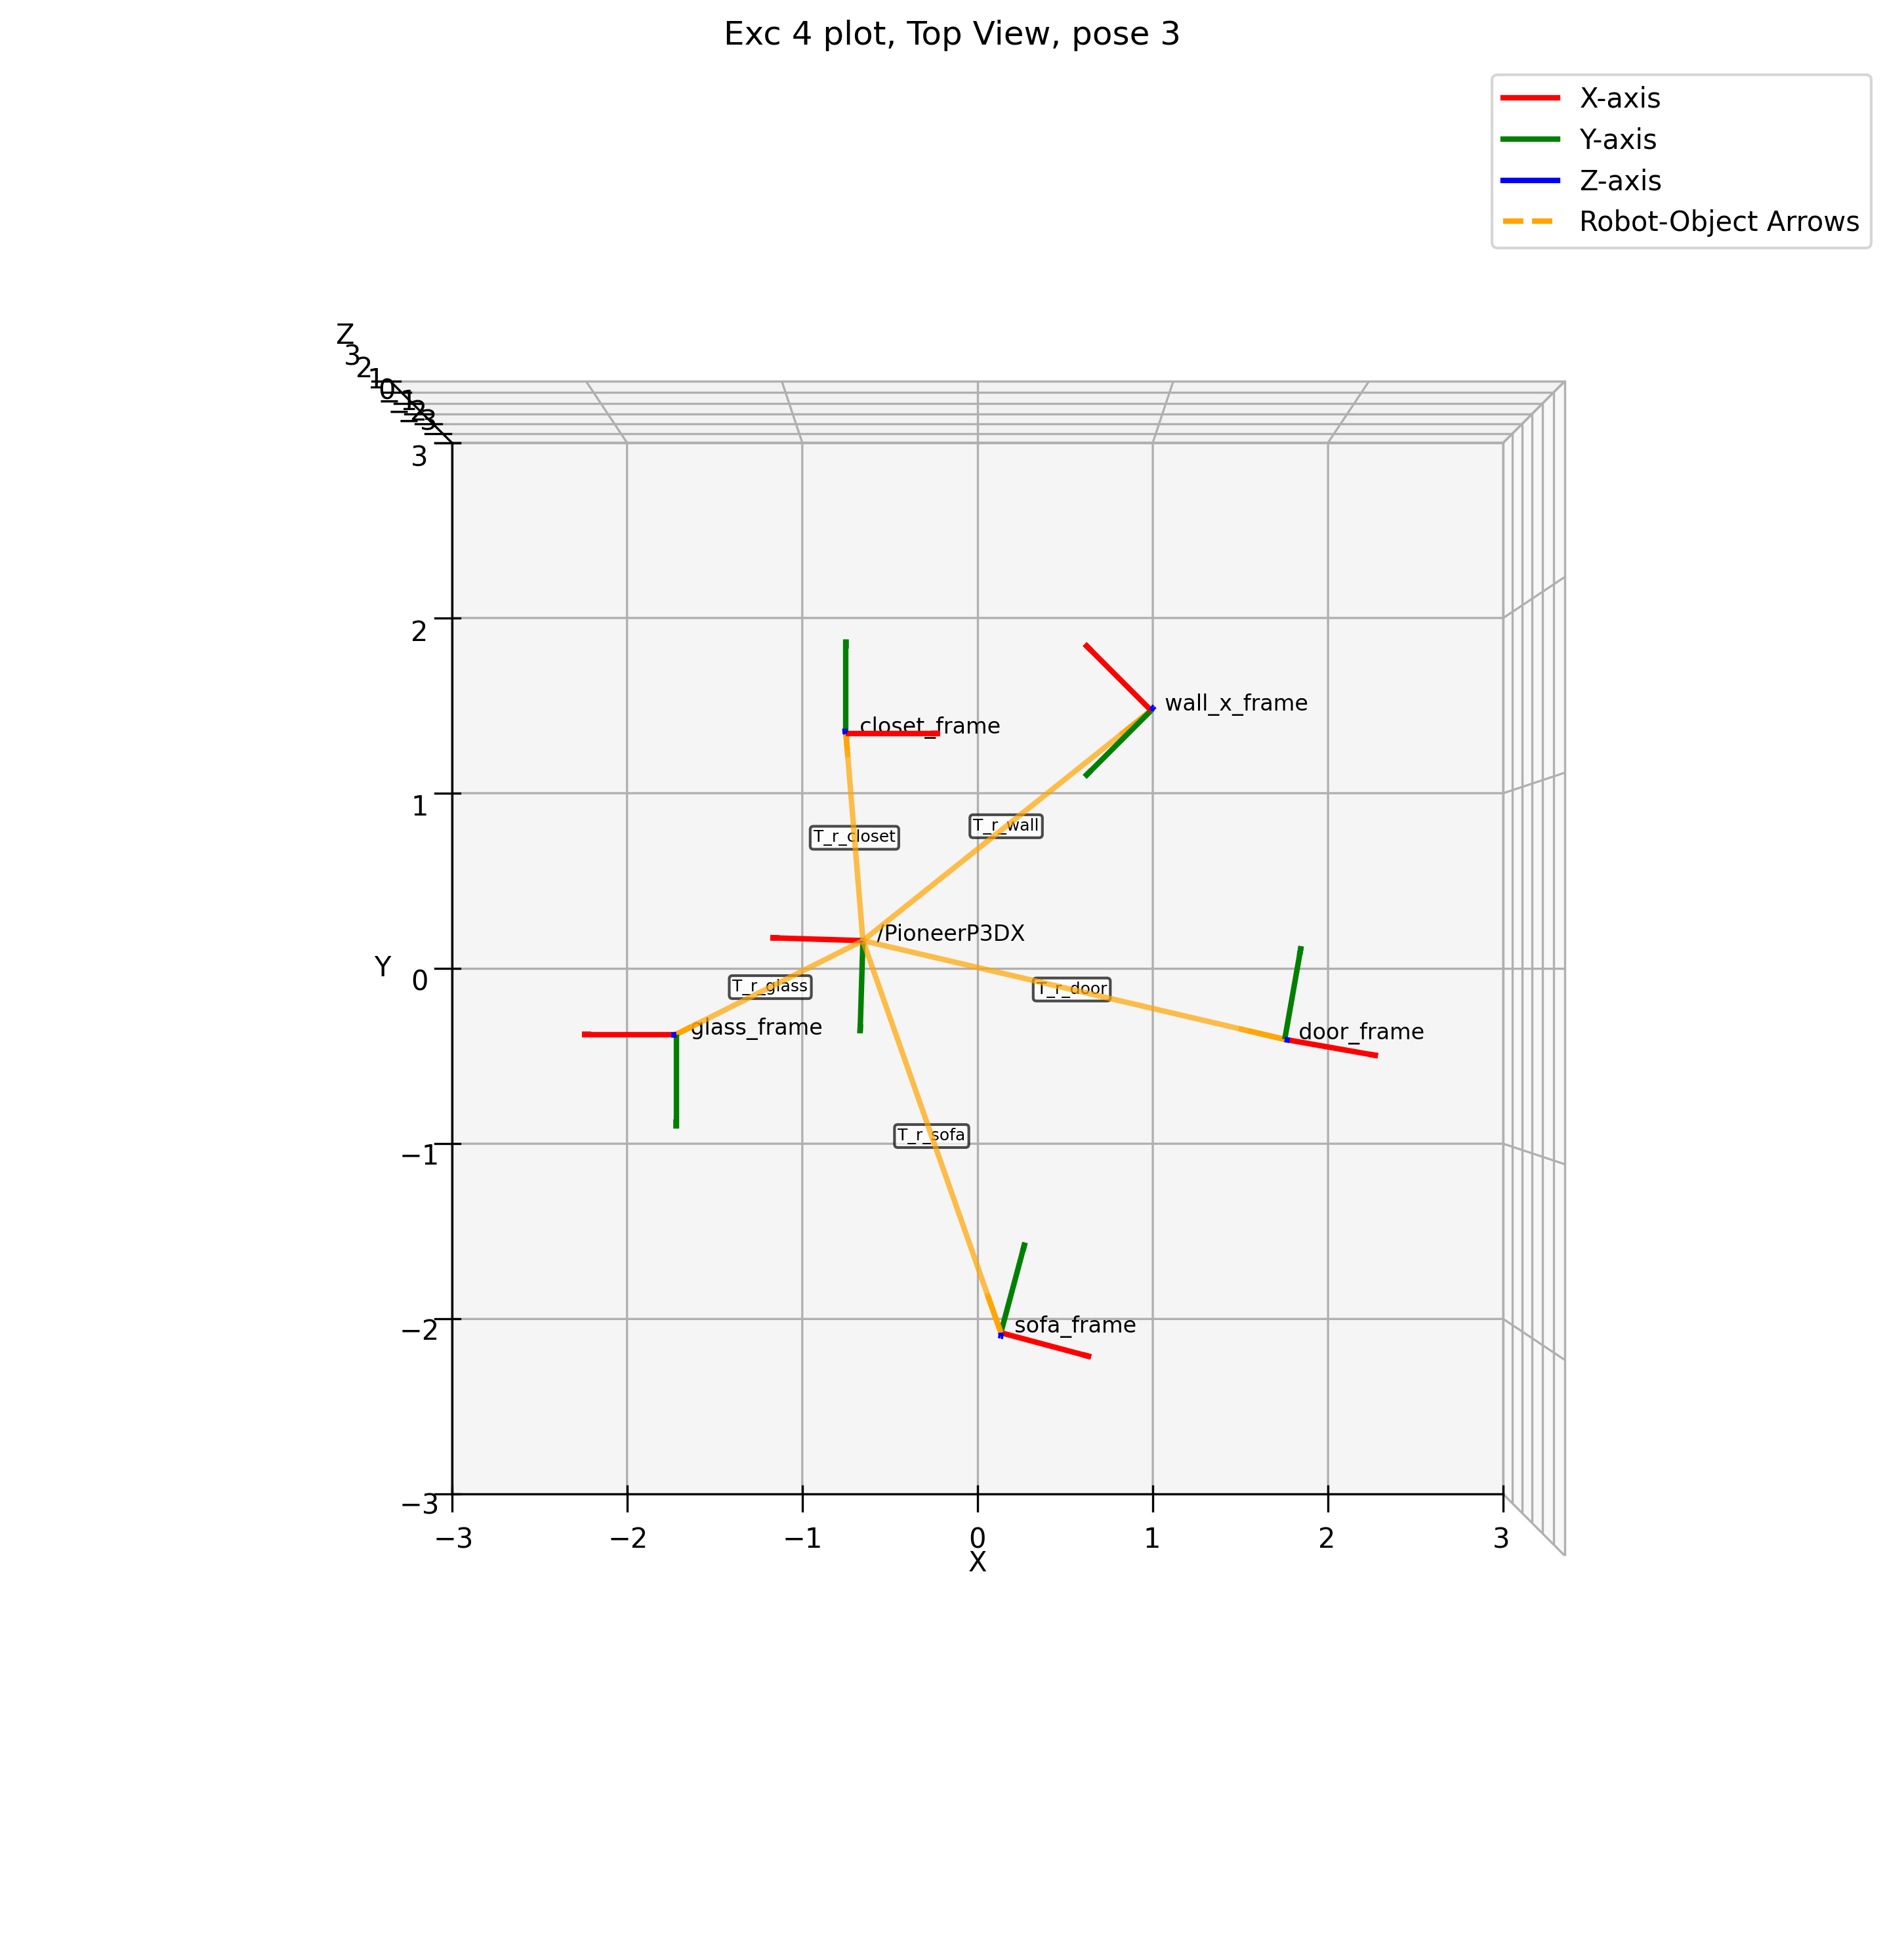
\includegraphics[width=\linewidth]{plots/q4_top_view_plot_3.png}
    \caption{Vista superior.}
    \label{fig:q4:a}
  \end{subfigure}\hfill
  \begin{subfigure}[t]{0.49\linewidth}
    \centering
    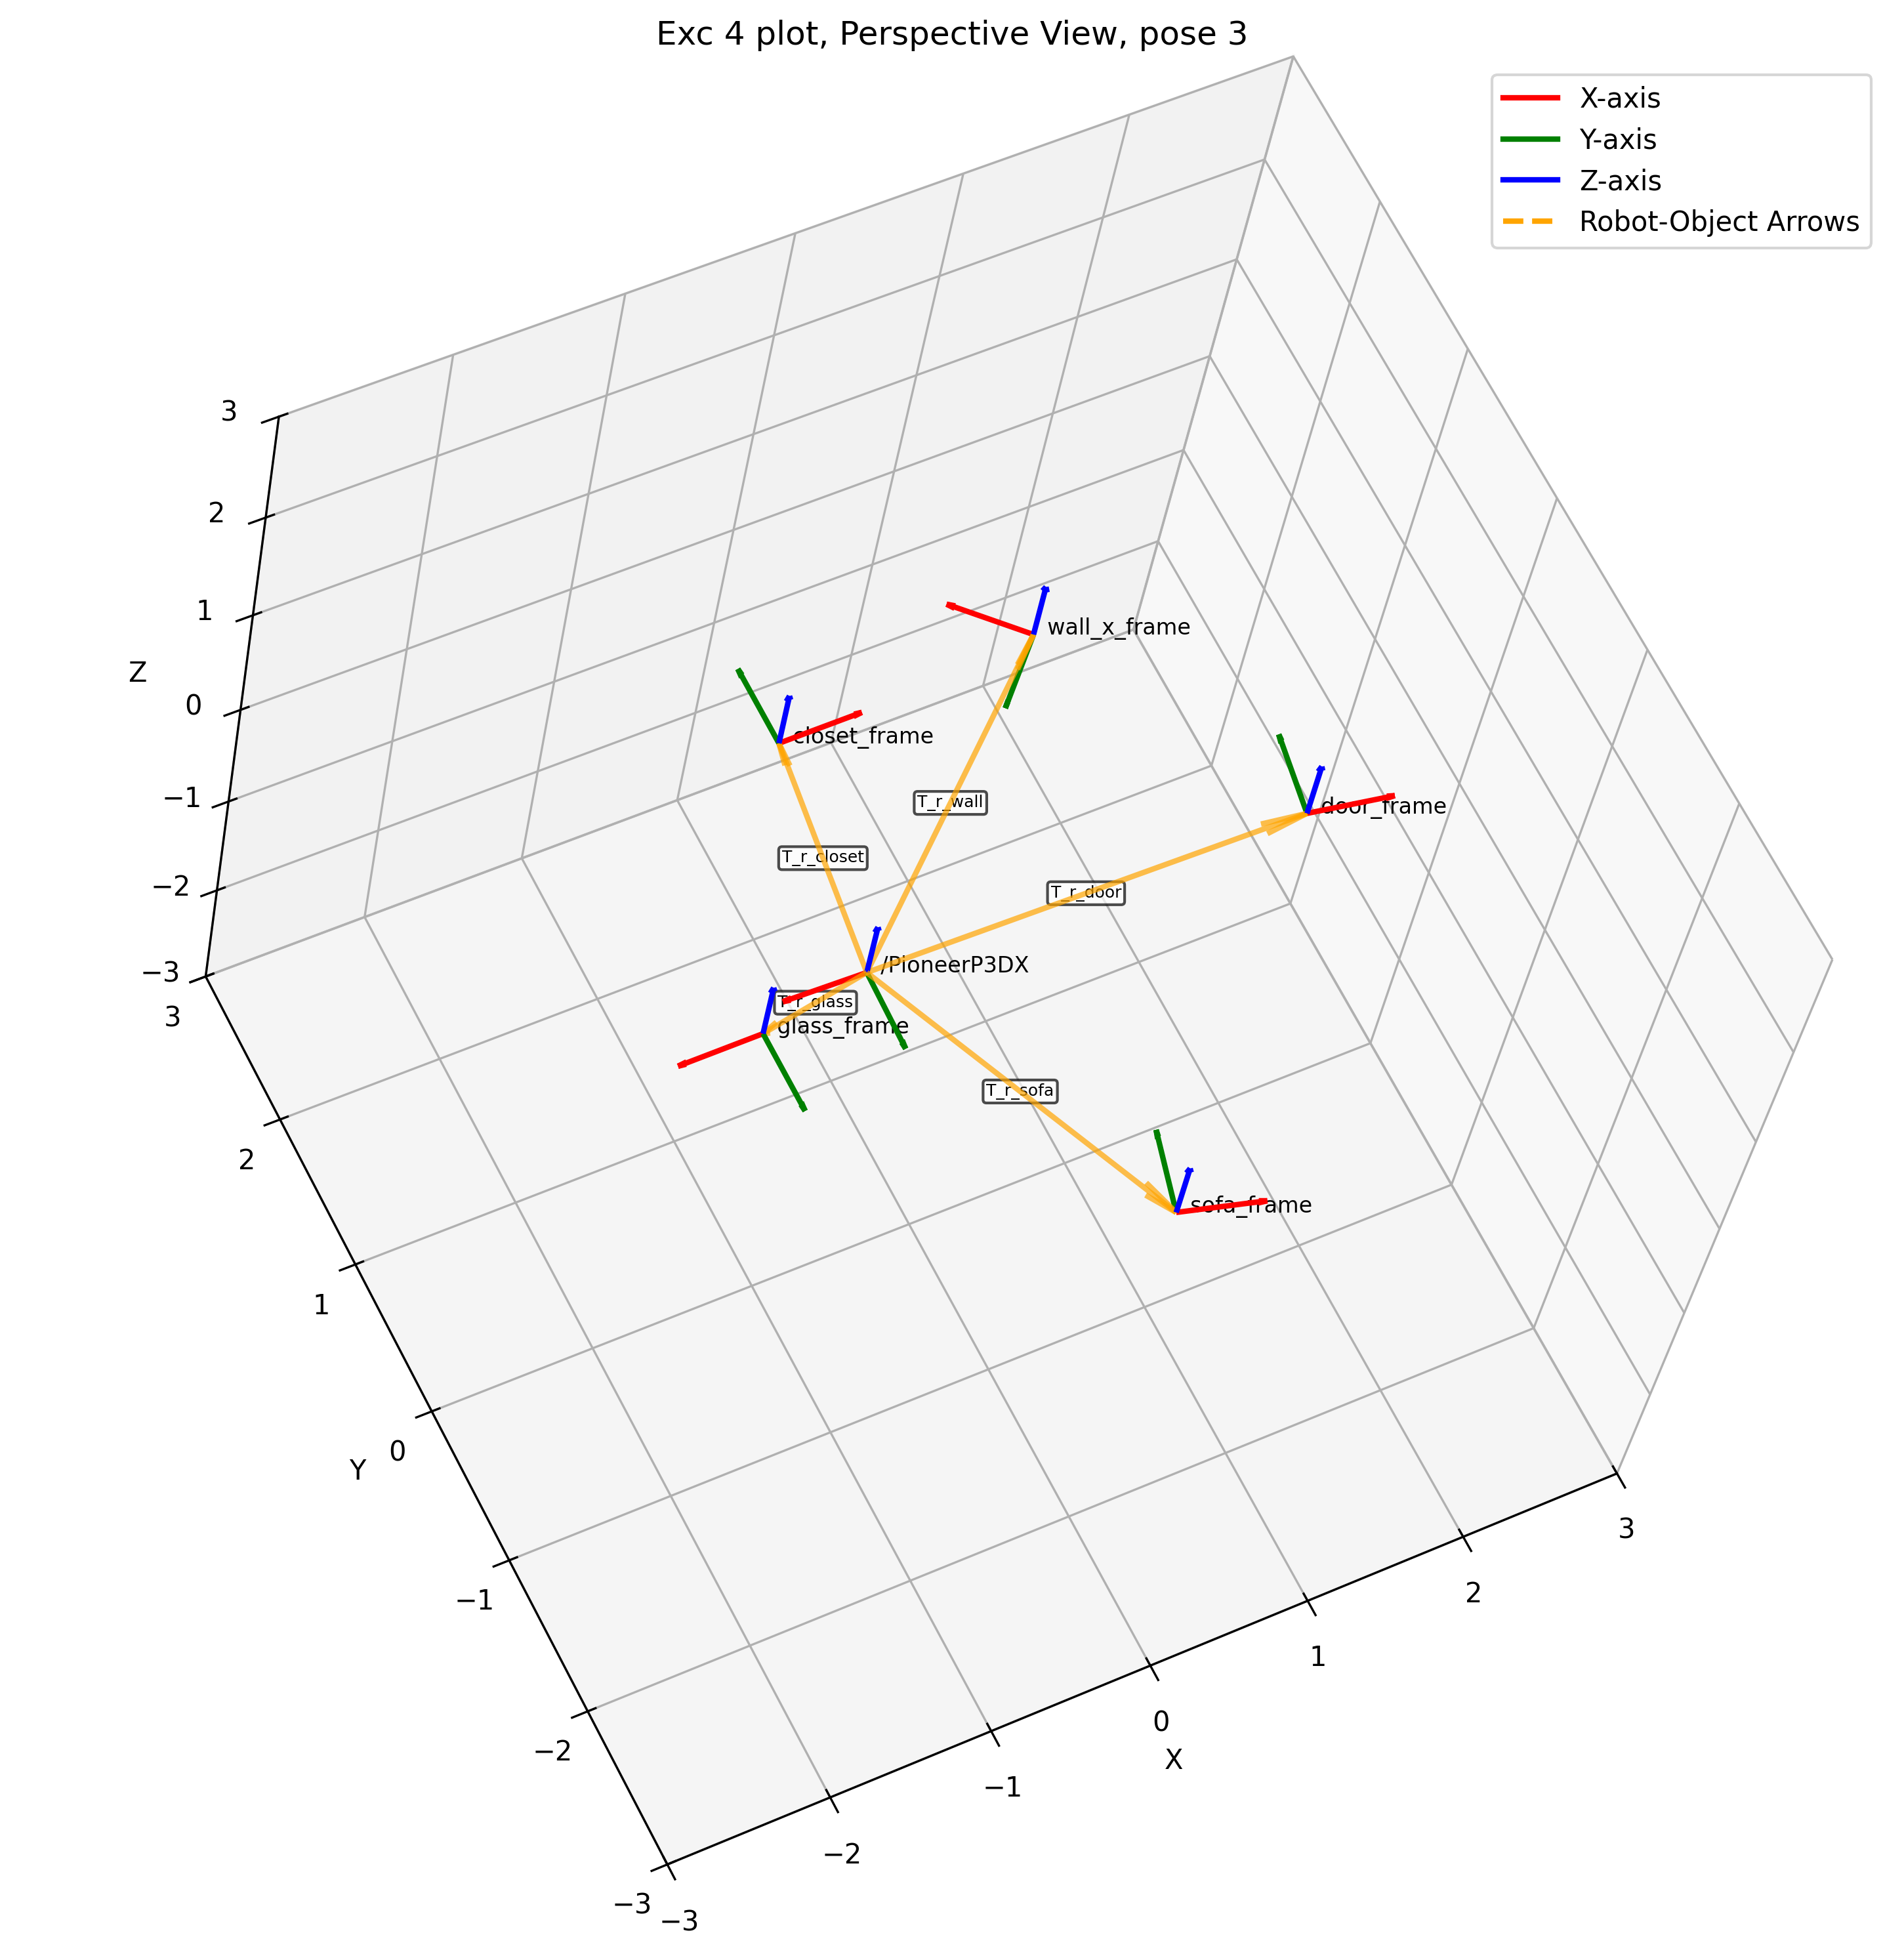
\includegraphics[width=\linewidth]{plots/q4_perspective_plot_3.png}
    \caption{Vista em perspectiva.}
    \label{fig:q4:b}
  \end{subfigure}
  \caption{Q4 - Resultados para pose 3 do robô.}
  \label{fig:q4}
\end{figure}

\noindent

\begin{tcolorbox}[enhanced,attach boxed title to top center={yshift=-3mm,yshifttext=-1mm}, colback=blue!5!white, colframe=blue!75!black, colbacktitle=blue!40!white, title=Homogeneous transforms for Random Pose 3,fonttitle=\bfseries, boxed title style={size=small,colframe=blue!50!black} ]
    \label{tab:q4_3}
    \begin{minipage}[t]{0.49\linewidth}
    \small
    \[
    \mat{T}^{W}_{R} =
    \begin{bmatrix}
     -0.99 & -0.14 & 0.00 & -0.85 \\
     0.14 & -0.99 & 0.00 & 0.11 \\
     0.00 &  0.00 & 1.00 & 0.14 \\
     0.00 &  0.00 & 0.00 & 1.00
    \end{bmatrix}
    \]
    \vspace{8pt}
    \[
    \mat{T}^{R}_{G} =
    \begin{bmatrix}
     0.99 & -0.14 & 0.00 & 0.68 \\
     0.14 &  0.99 & 0.00 & 0.56 \\
     0.00 &  0.00 & 1.00 & 0.86 \\
     0.00 &  0.00 & 0.00 & 1.00
    \end{bmatrix}
    \]
    \vspace{8pt}
    \[
    \mat{T}^{R}_{D} =
    \begin{bmatrix}
     -1.00 & -0.04 & 0.00 & -2.52 \\
      0.04 & -1.00 & 0.00 &  0.14 \\
      0.00 &  0.00 & 1.00 &  1.06 \\
      0.00 &  0.00 & 0.00 &  1.00
    \end{bmatrix}
    \]
    \end{minipage}\hfill
    \begin{minipage}[t]{0.49\linewidth}
    \small
    \[
    \mat{T}^{R}_{C} =
    \begin{bmatrix}
     -0.99 &  0.14 & 0.00 &  0.01 \\
     -0.14 & -0.99 & 0.00 & -1.15 \\
      0.00 &  0.00 & 1.00 &  0.76 \\
      0.00 &  0.00 & 0.00 &  1.00
    \end{bmatrix}
    \]
    \vspace{8pt}
    \[
    \mat{T}^{R}_{S} =
    \begin{bmatrix}
     -0.99 & -0.12 & 0.00 & -1.25 \\
      0.12 & -0.99 & 0.00 &  1.91 \\
      0.00 &  0.00 & 1.00 &  0.36 \\
      0.00 &  0.00 & 0.00 &  1.00
    \end{bmatrix}
    \]
    \vspace{8pt}
    \[
    \mat{T}^{R}_{X} =
    \begin{bmatrix}
      0.80 &  0.60 & 0.00 & -1.59 \\
     -0.60 &  0.80 & 0.00 & -1.50 \\
      0.00 &  0.00 & 1.00 &  0.66 \\
      0.00 &  0.00 & 0.00 &  1.00
    \end{bmatrix}
    \]
    \end{minipage}
\end{tcolorbox}

% ============================
\section*{Questão 5 \ \textnormal{[1,5 pts]}}
\textbf{Enunciado.}
Substitua o robô adicionado inicialmente na cena pelo robô com laser mostrado em aula. No exemplo que vimos, o plot da leitura do laser está sendo feito no referencial local do laser. Defina as matrizes de transformações \(T_{L\rightarrow R}\) (laser \(\rightarrow\) robô) e \(T_{R\rightarrow W}\) (robô \(\rightarrow\) mundo), e em seguida modifique o script original para que os pontos agora sejam plotados no referencial global, de acordo com a posição atual do robô (recuperada pela RemoteAPI). Coloque o robô em outras diferentes posições da cena (e.g., três) e faça os plots das leituras do laser.

\vspace{6pt}
\textbf{Resposta.}
Sejam \(\mat{T}^{R}_{L} = T_{L\rightarrow R}\) e \(\mat{T}^{W}_{R} = T_{R\rightarrow W}\). A transformação composta do laser para o mundo é
\[
\mat{T}^{W}_{L} \;=\; \mat{T}^{W}_{R}\, \mat{T}^{R}_{L}.
\]
Para cada ponto do feixe do laser expresso em coordenadas do laser, \(\tilde{\vect{p}}_{L} = [x\ y\ 0\ 1]^\top\), o ponto no mundo é
\[
\tilde{\vect{p}}_{W} = \mat{T}^{W}_{L}\, \tilde{\vect{p}}_{L}.
\]
O script atualiza \(\mat{T}^{W}_{R}\) a cada pose do robô obtida via RemoteAPI e plota as leituras já em \(W\). Foram testadas três poses distintas:
\begin{figure}[H]
  \centering
  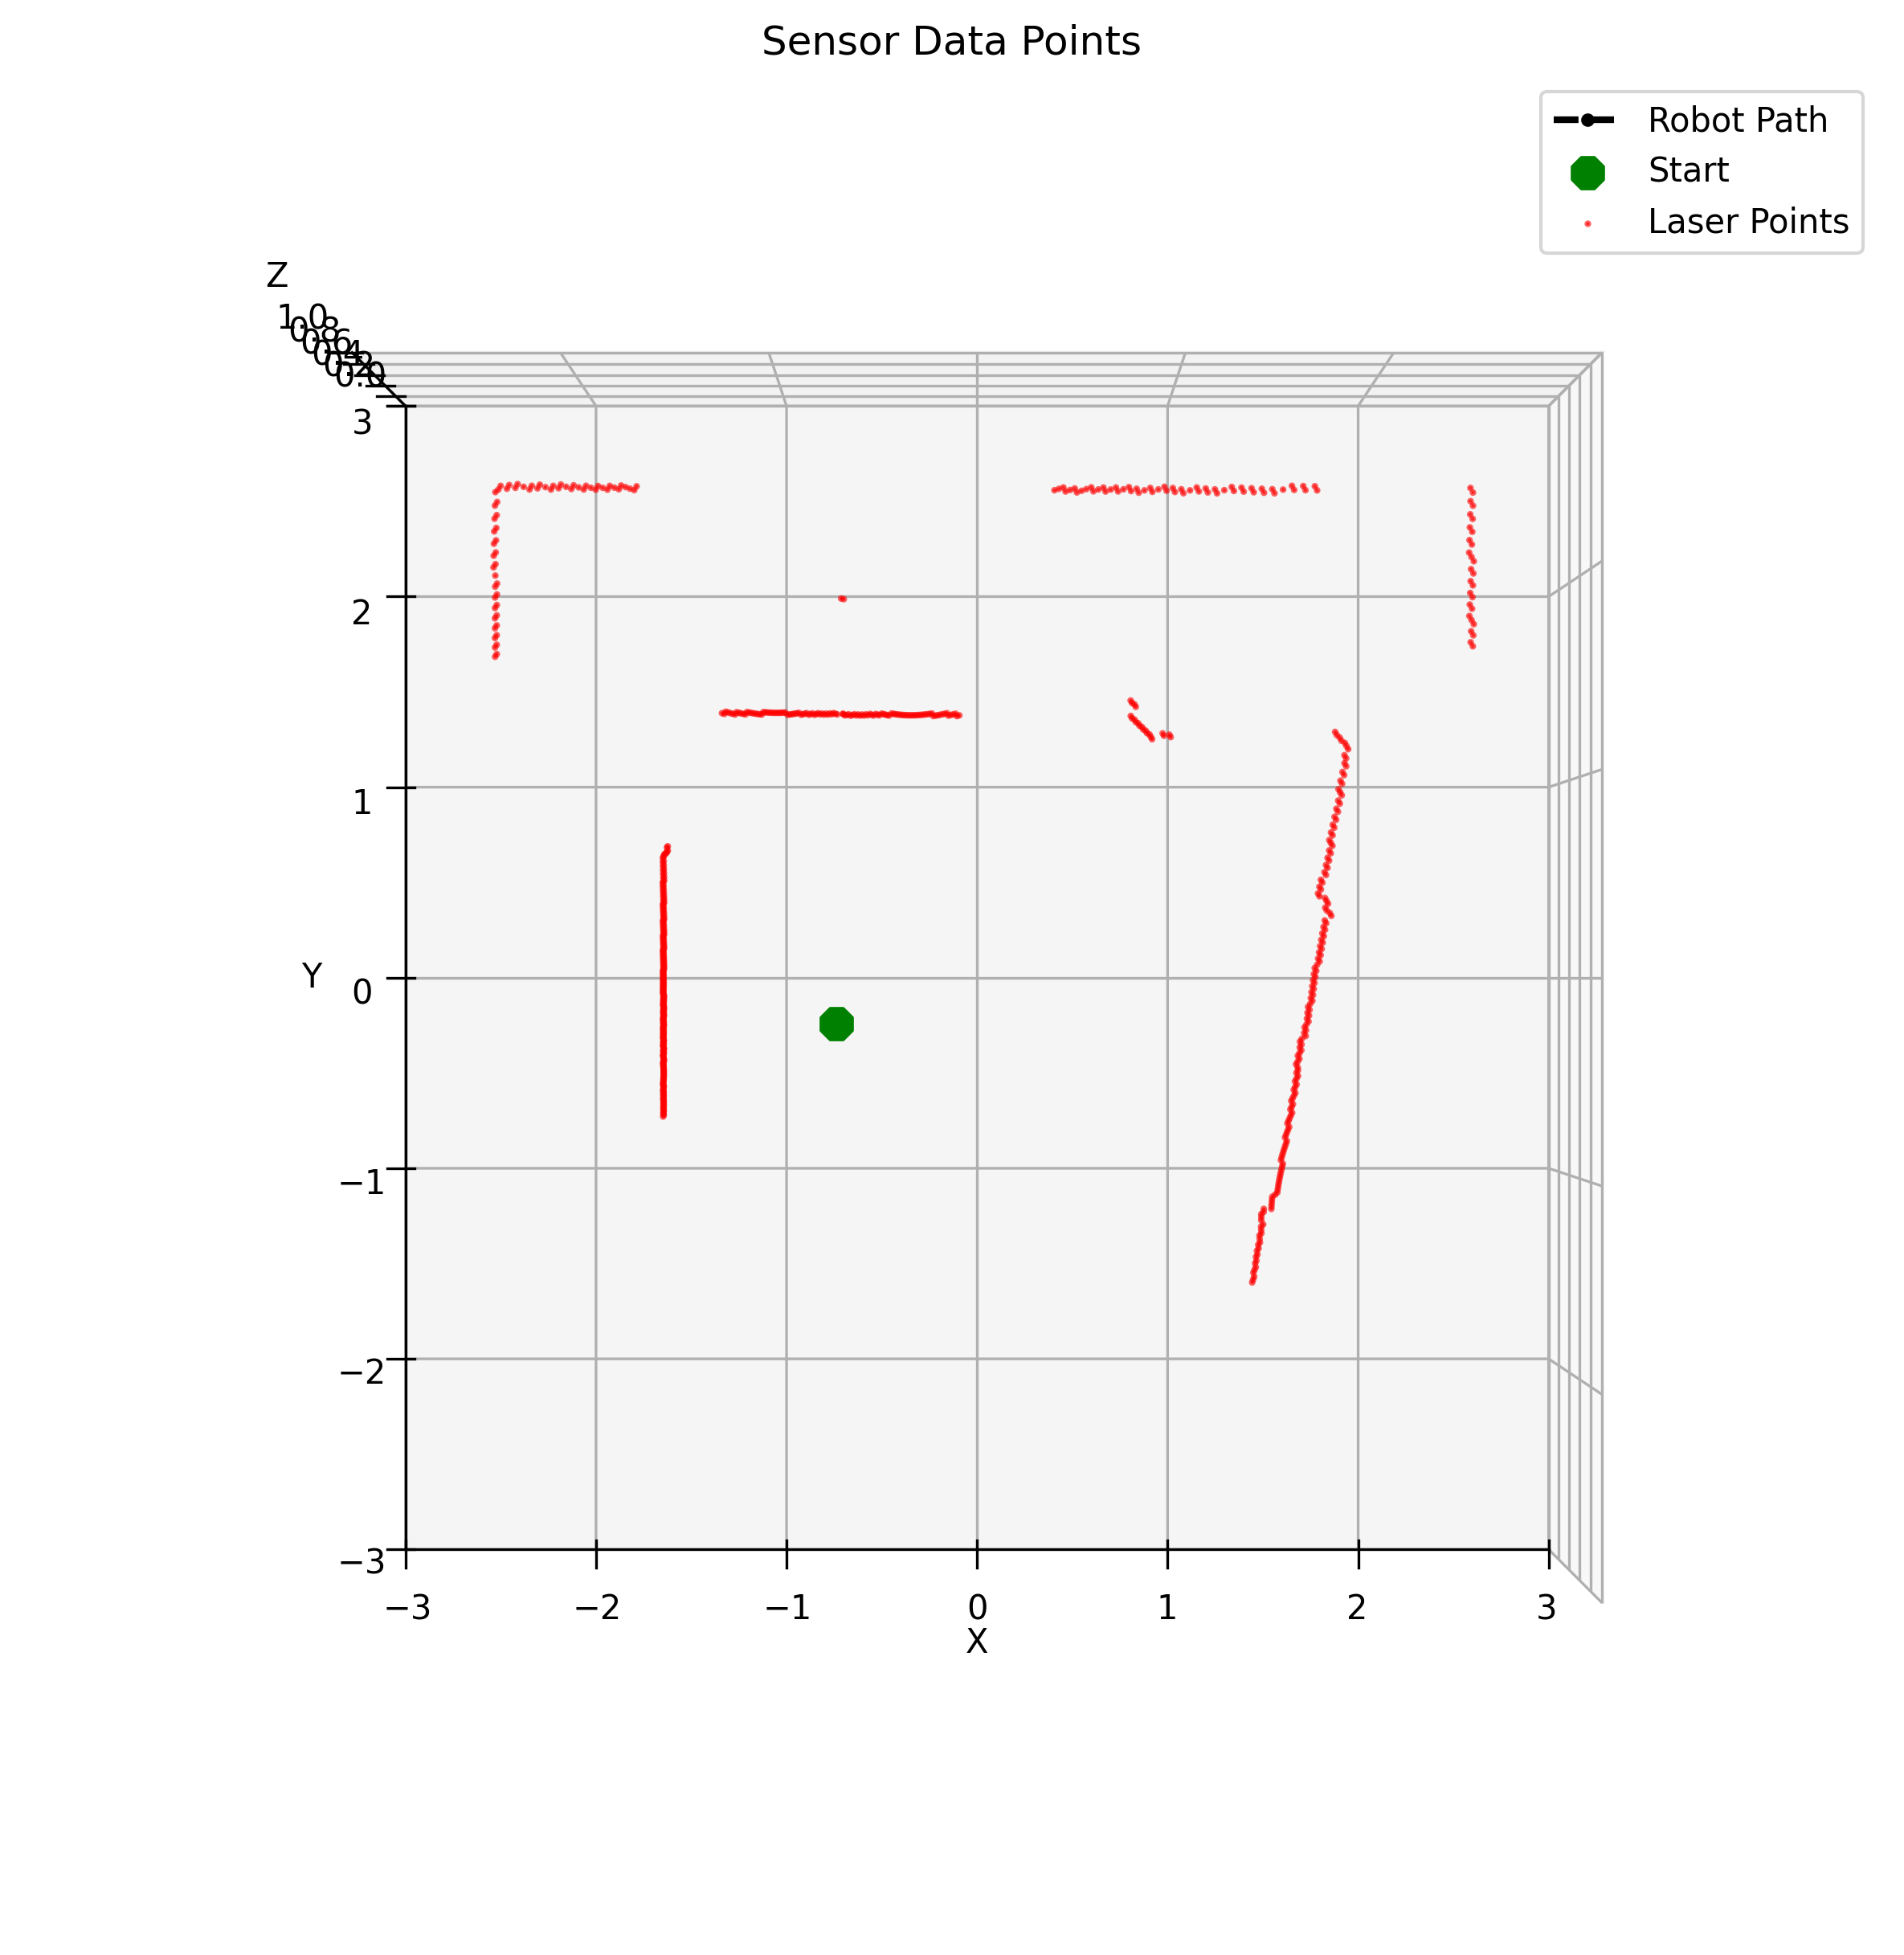
\includegraphics[width=\linewidth]{plots/q5_plot_1.png}
  \caption{Pose aleatória 1 - Leituras do laser no referencial global \(W\)}
\end{figure}

\begin{figure}[H]
  \centering
  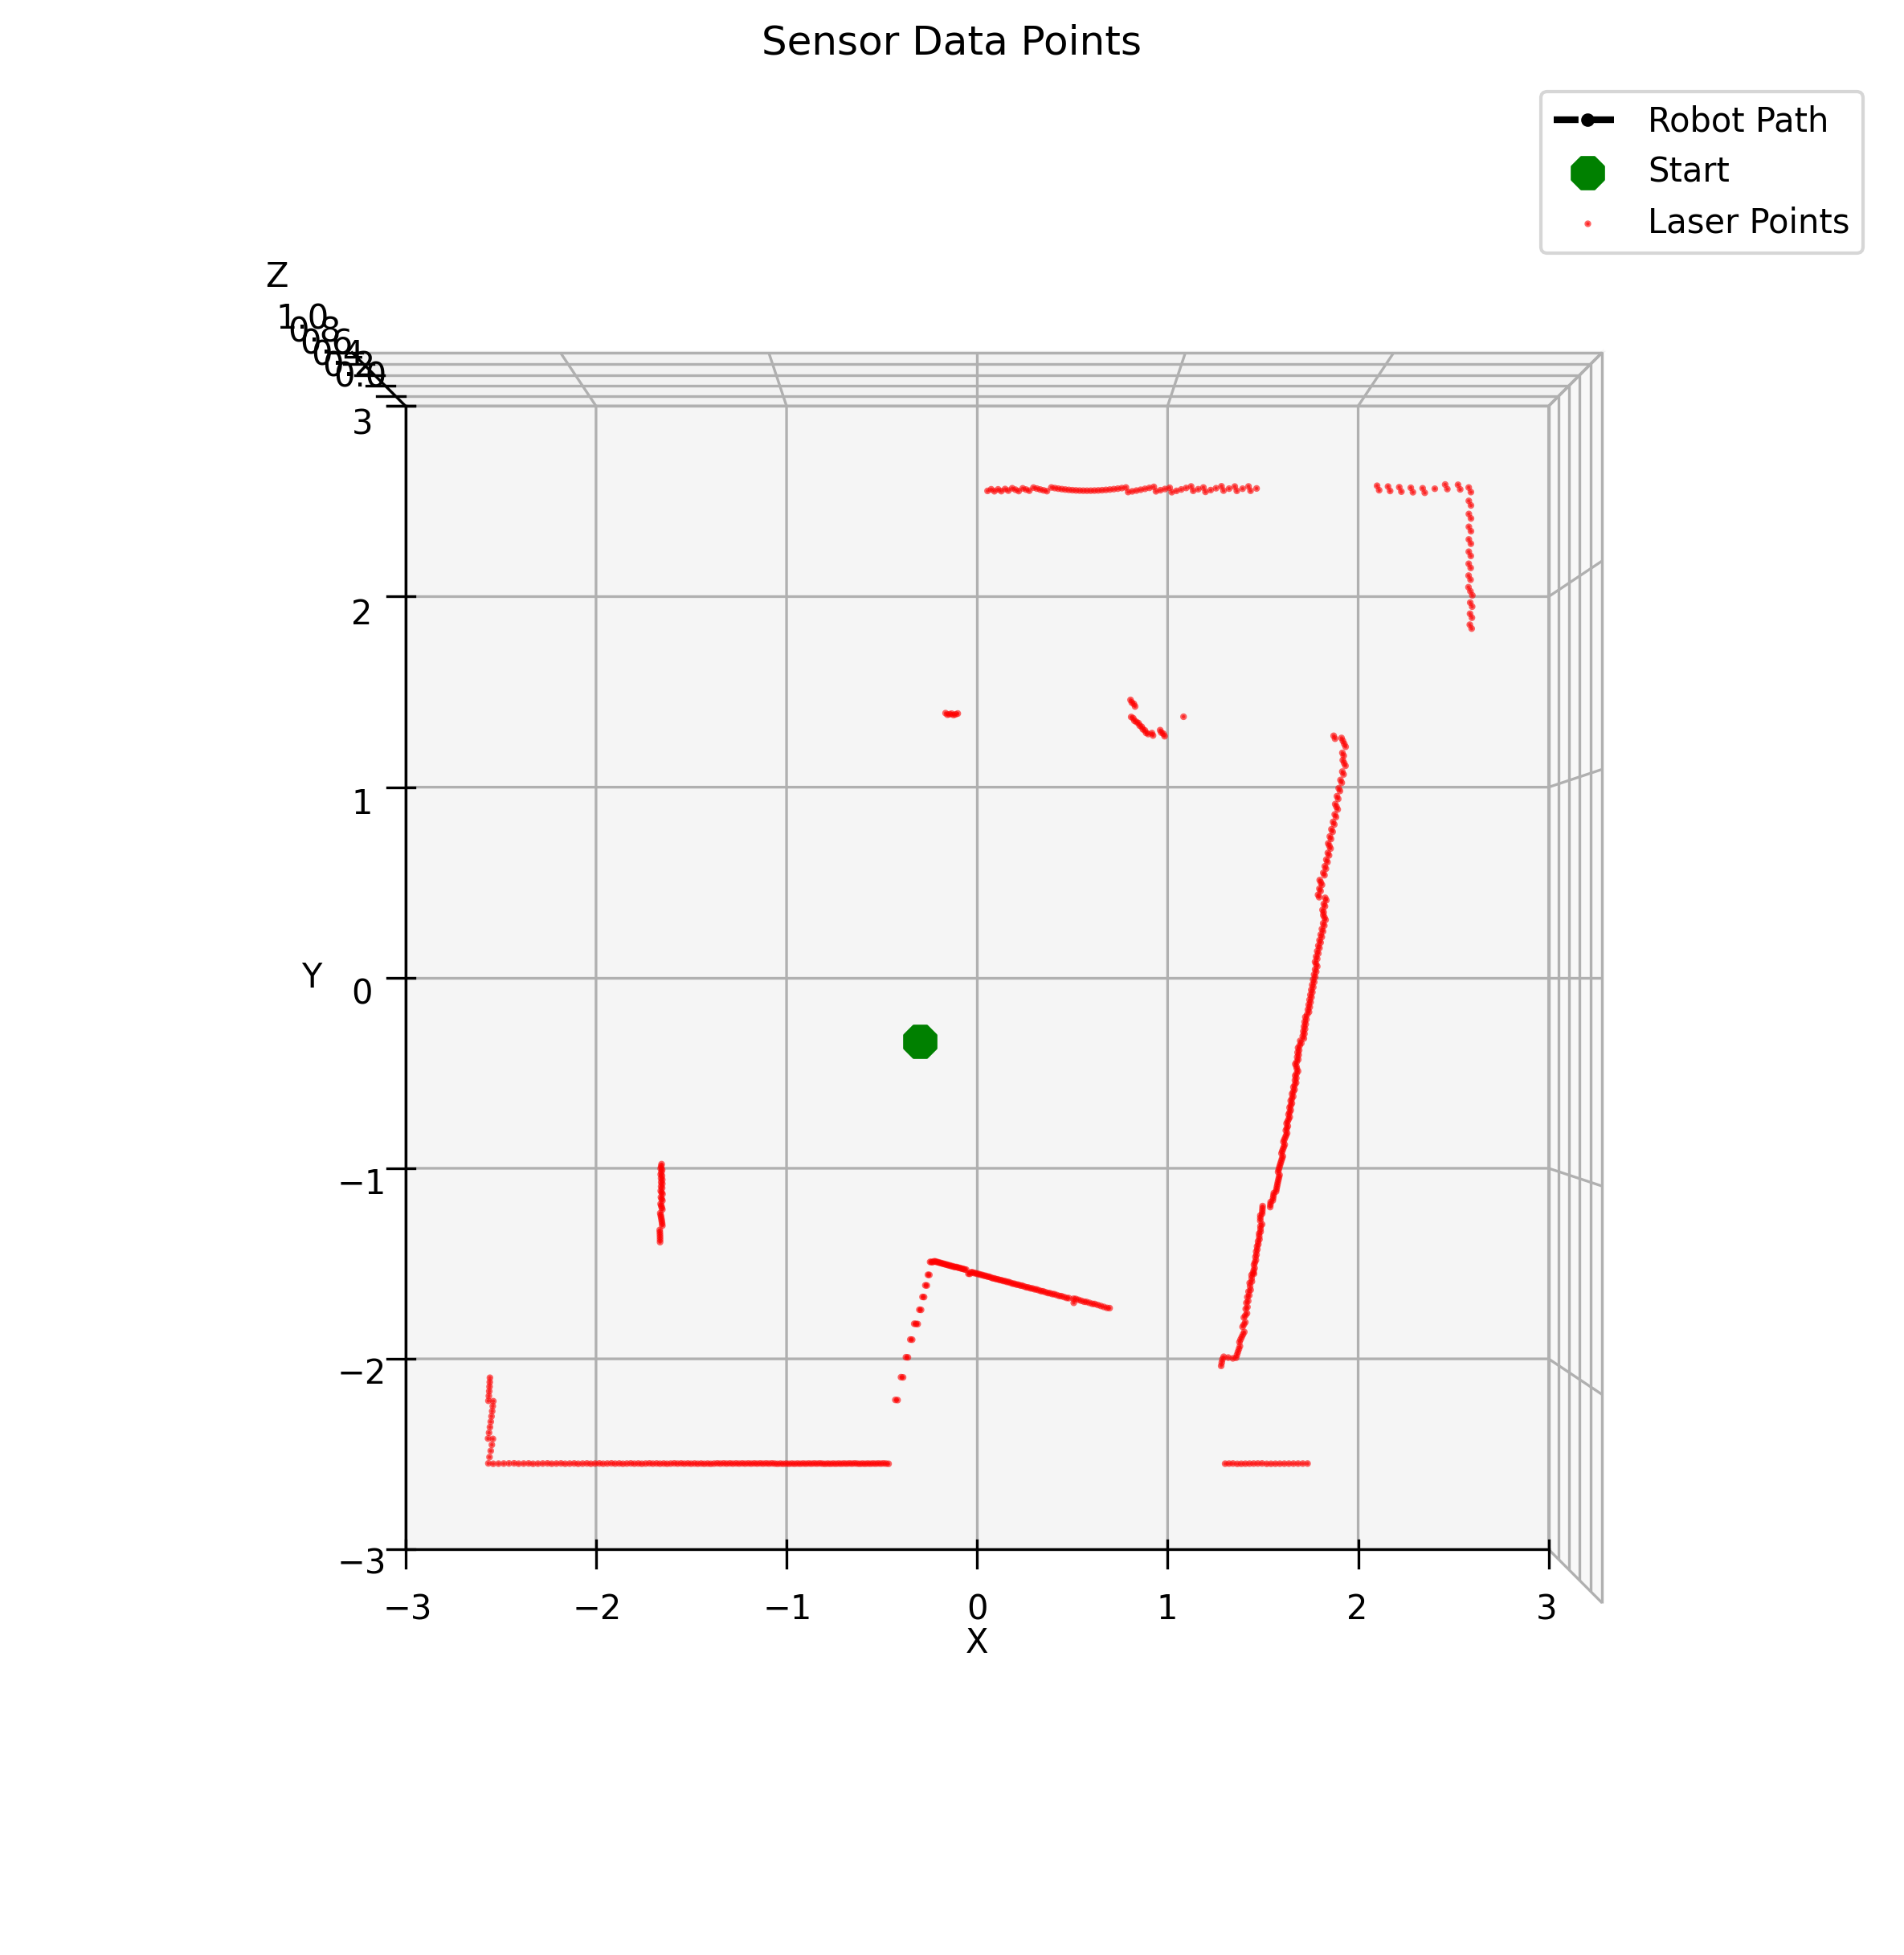
\includegraphics[width=\linewidth]{plots/q5_plot_2.png}
  \caption{Pose aleatória 2 - Leituras do laser no referencial global \(W\)}
\end{figure}

\begin{figure}[H]
  \centering
  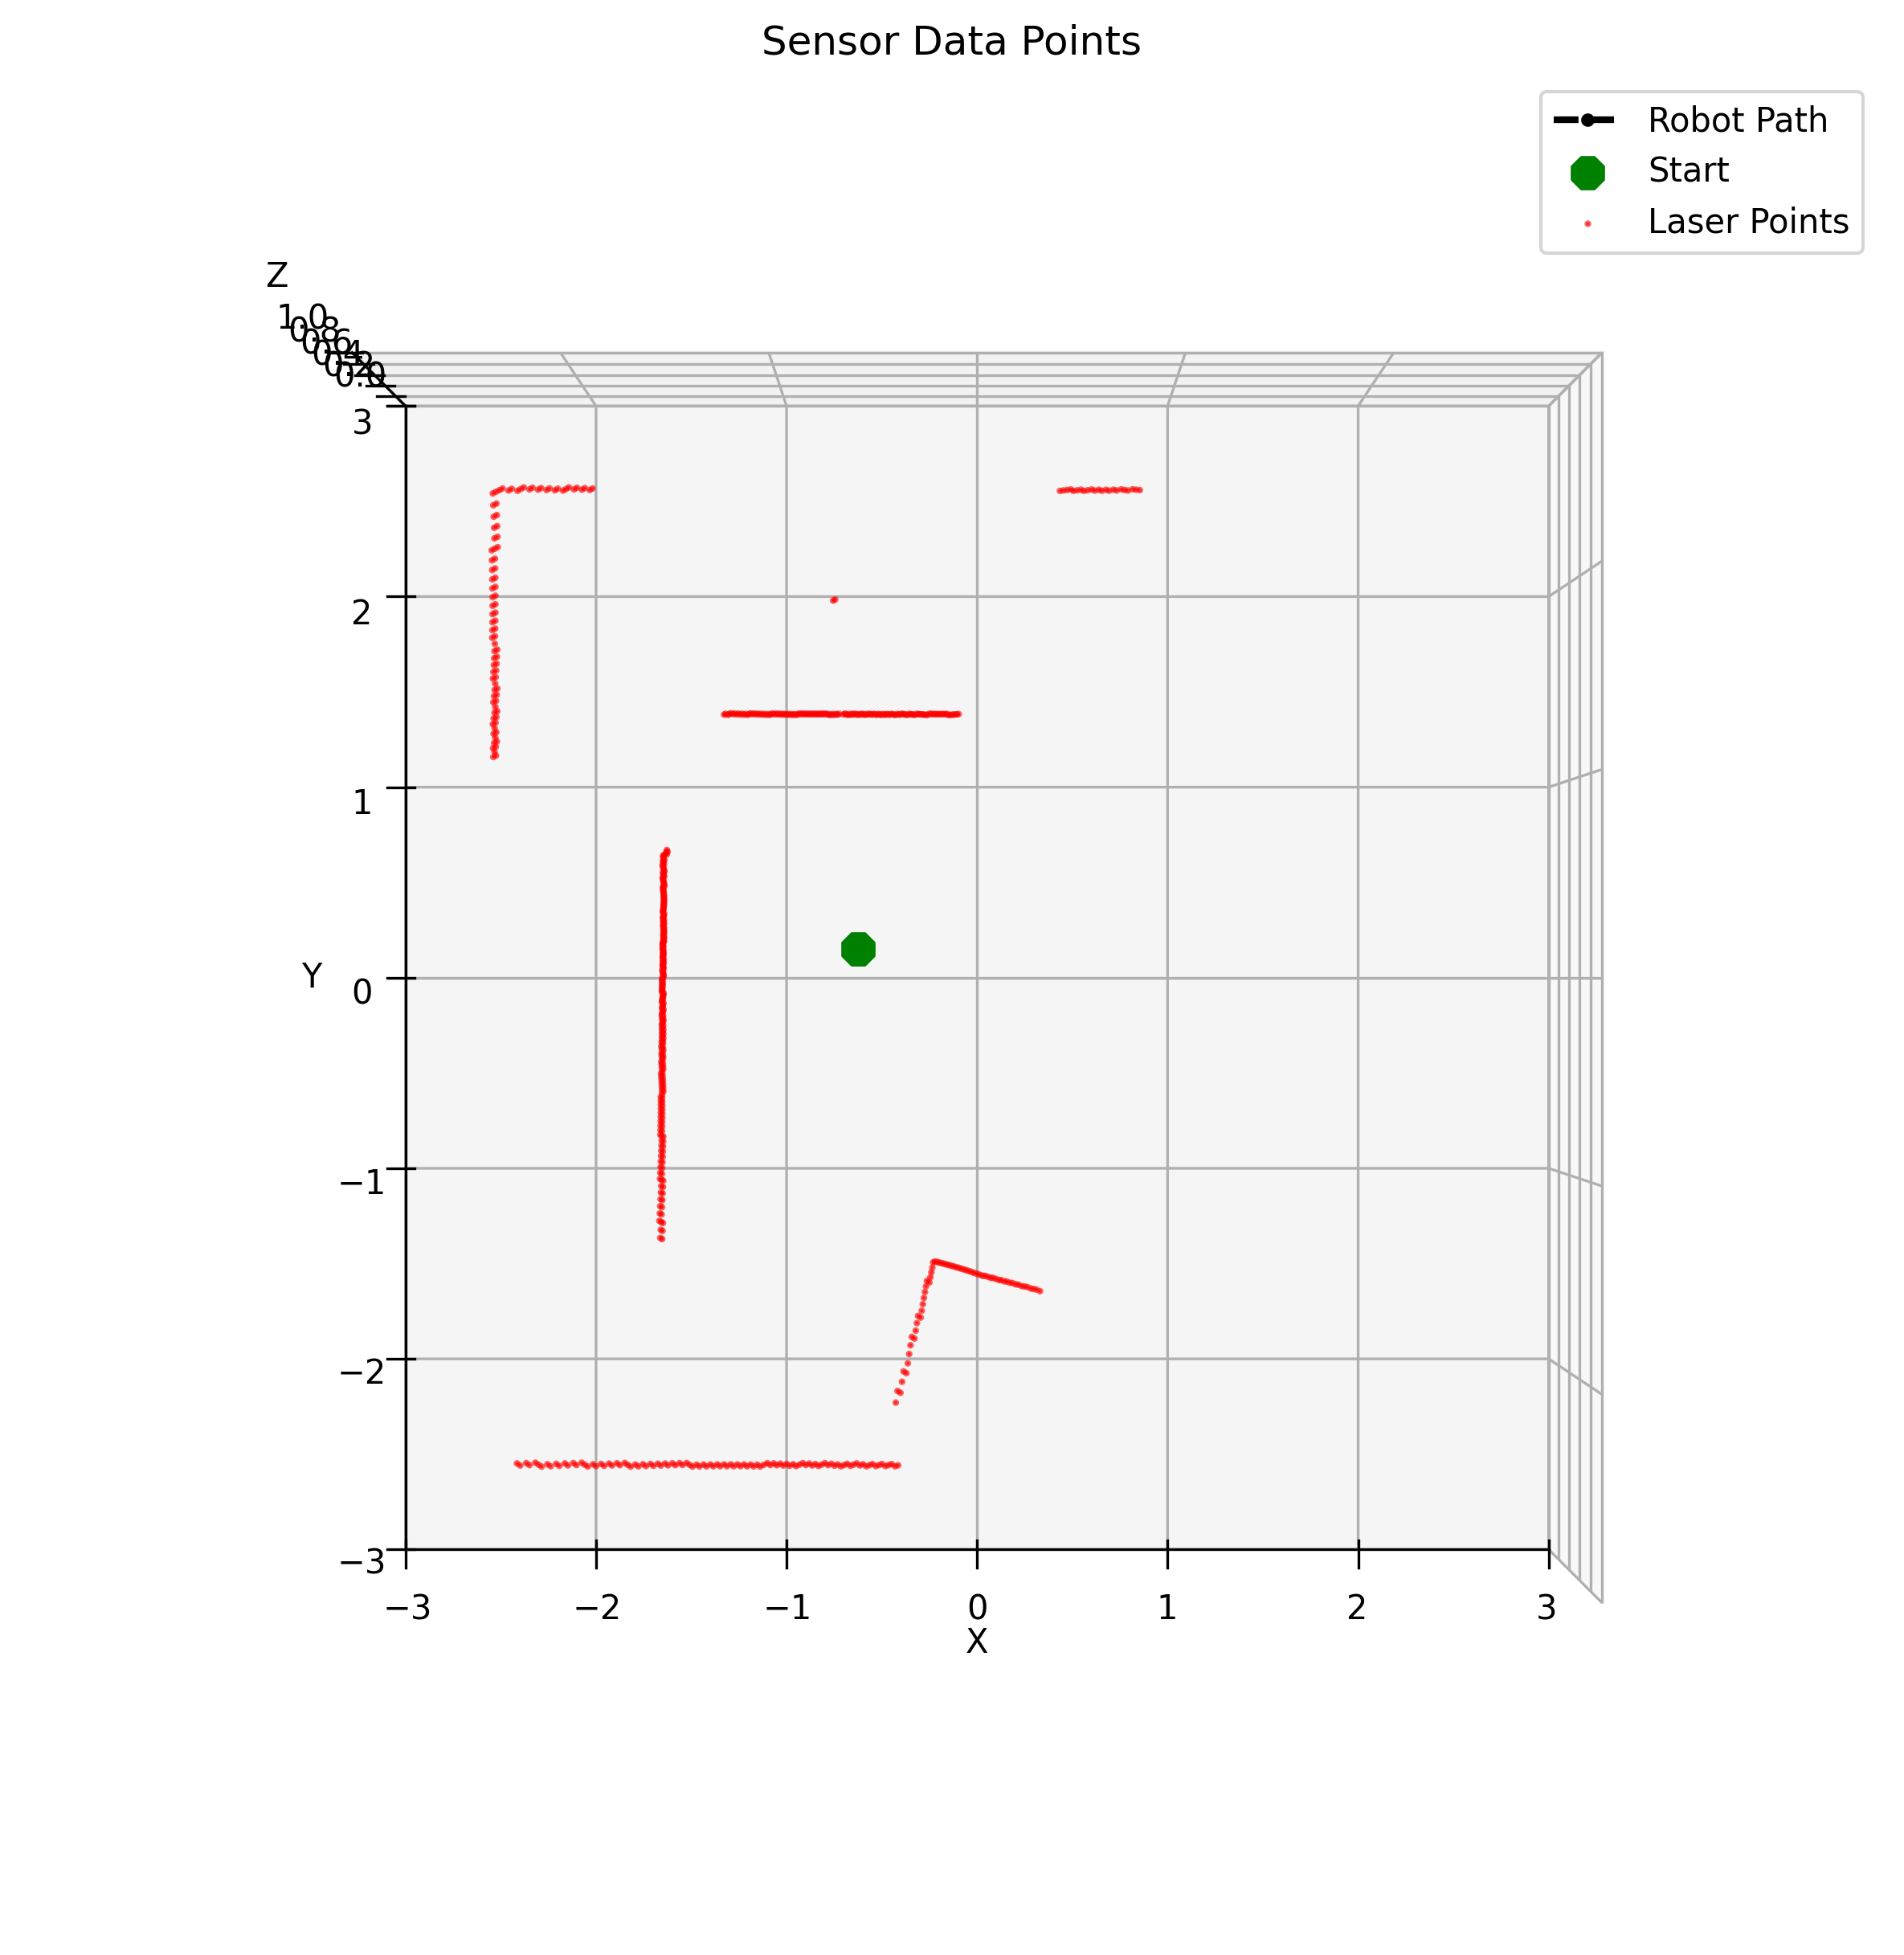
\includegraphics[width=\linewidth]{plots/q5_plot_3.png}
  \caption{Pose aleatória 3 - Leituras do laser no referencial global \(W\)}
\end{figure}

% ============================
\section*{Questão 6 \ \textnormal{[2,0 pts]}}
\textbf{Enunciado.}
Por fim, utilizando o script básico de navegação visto em aula, faça um plot incremental que mostra o caminho executado pelo robô (sequência de posições) ao longo da navegação (por exemplo, usando uma linha tracejada) e combina todas as leituras de laser realizadas ao longo do trajeto. Essas informações devem ser todas representadas em um único gráfico considerando o referencial global.

\vspace{6pt}
\textbf{Resposta.}
Durante a navegação, registra-se a trajetória do robô como \(\{(x_t,y_t,\theta_t)\}_t\) e, para cada varredura do laser, transforma-se os pontos para o mundo com \(\mat{T}^{W}_{L}(t)=\mat{T}^{W}_{R}(t)\mat{T}^{R}_{L}\).
Plota-se a trajetória com linha tracejada e sobrepõem-se todas as leituras:
\begin{figure}[H]
  \centering
  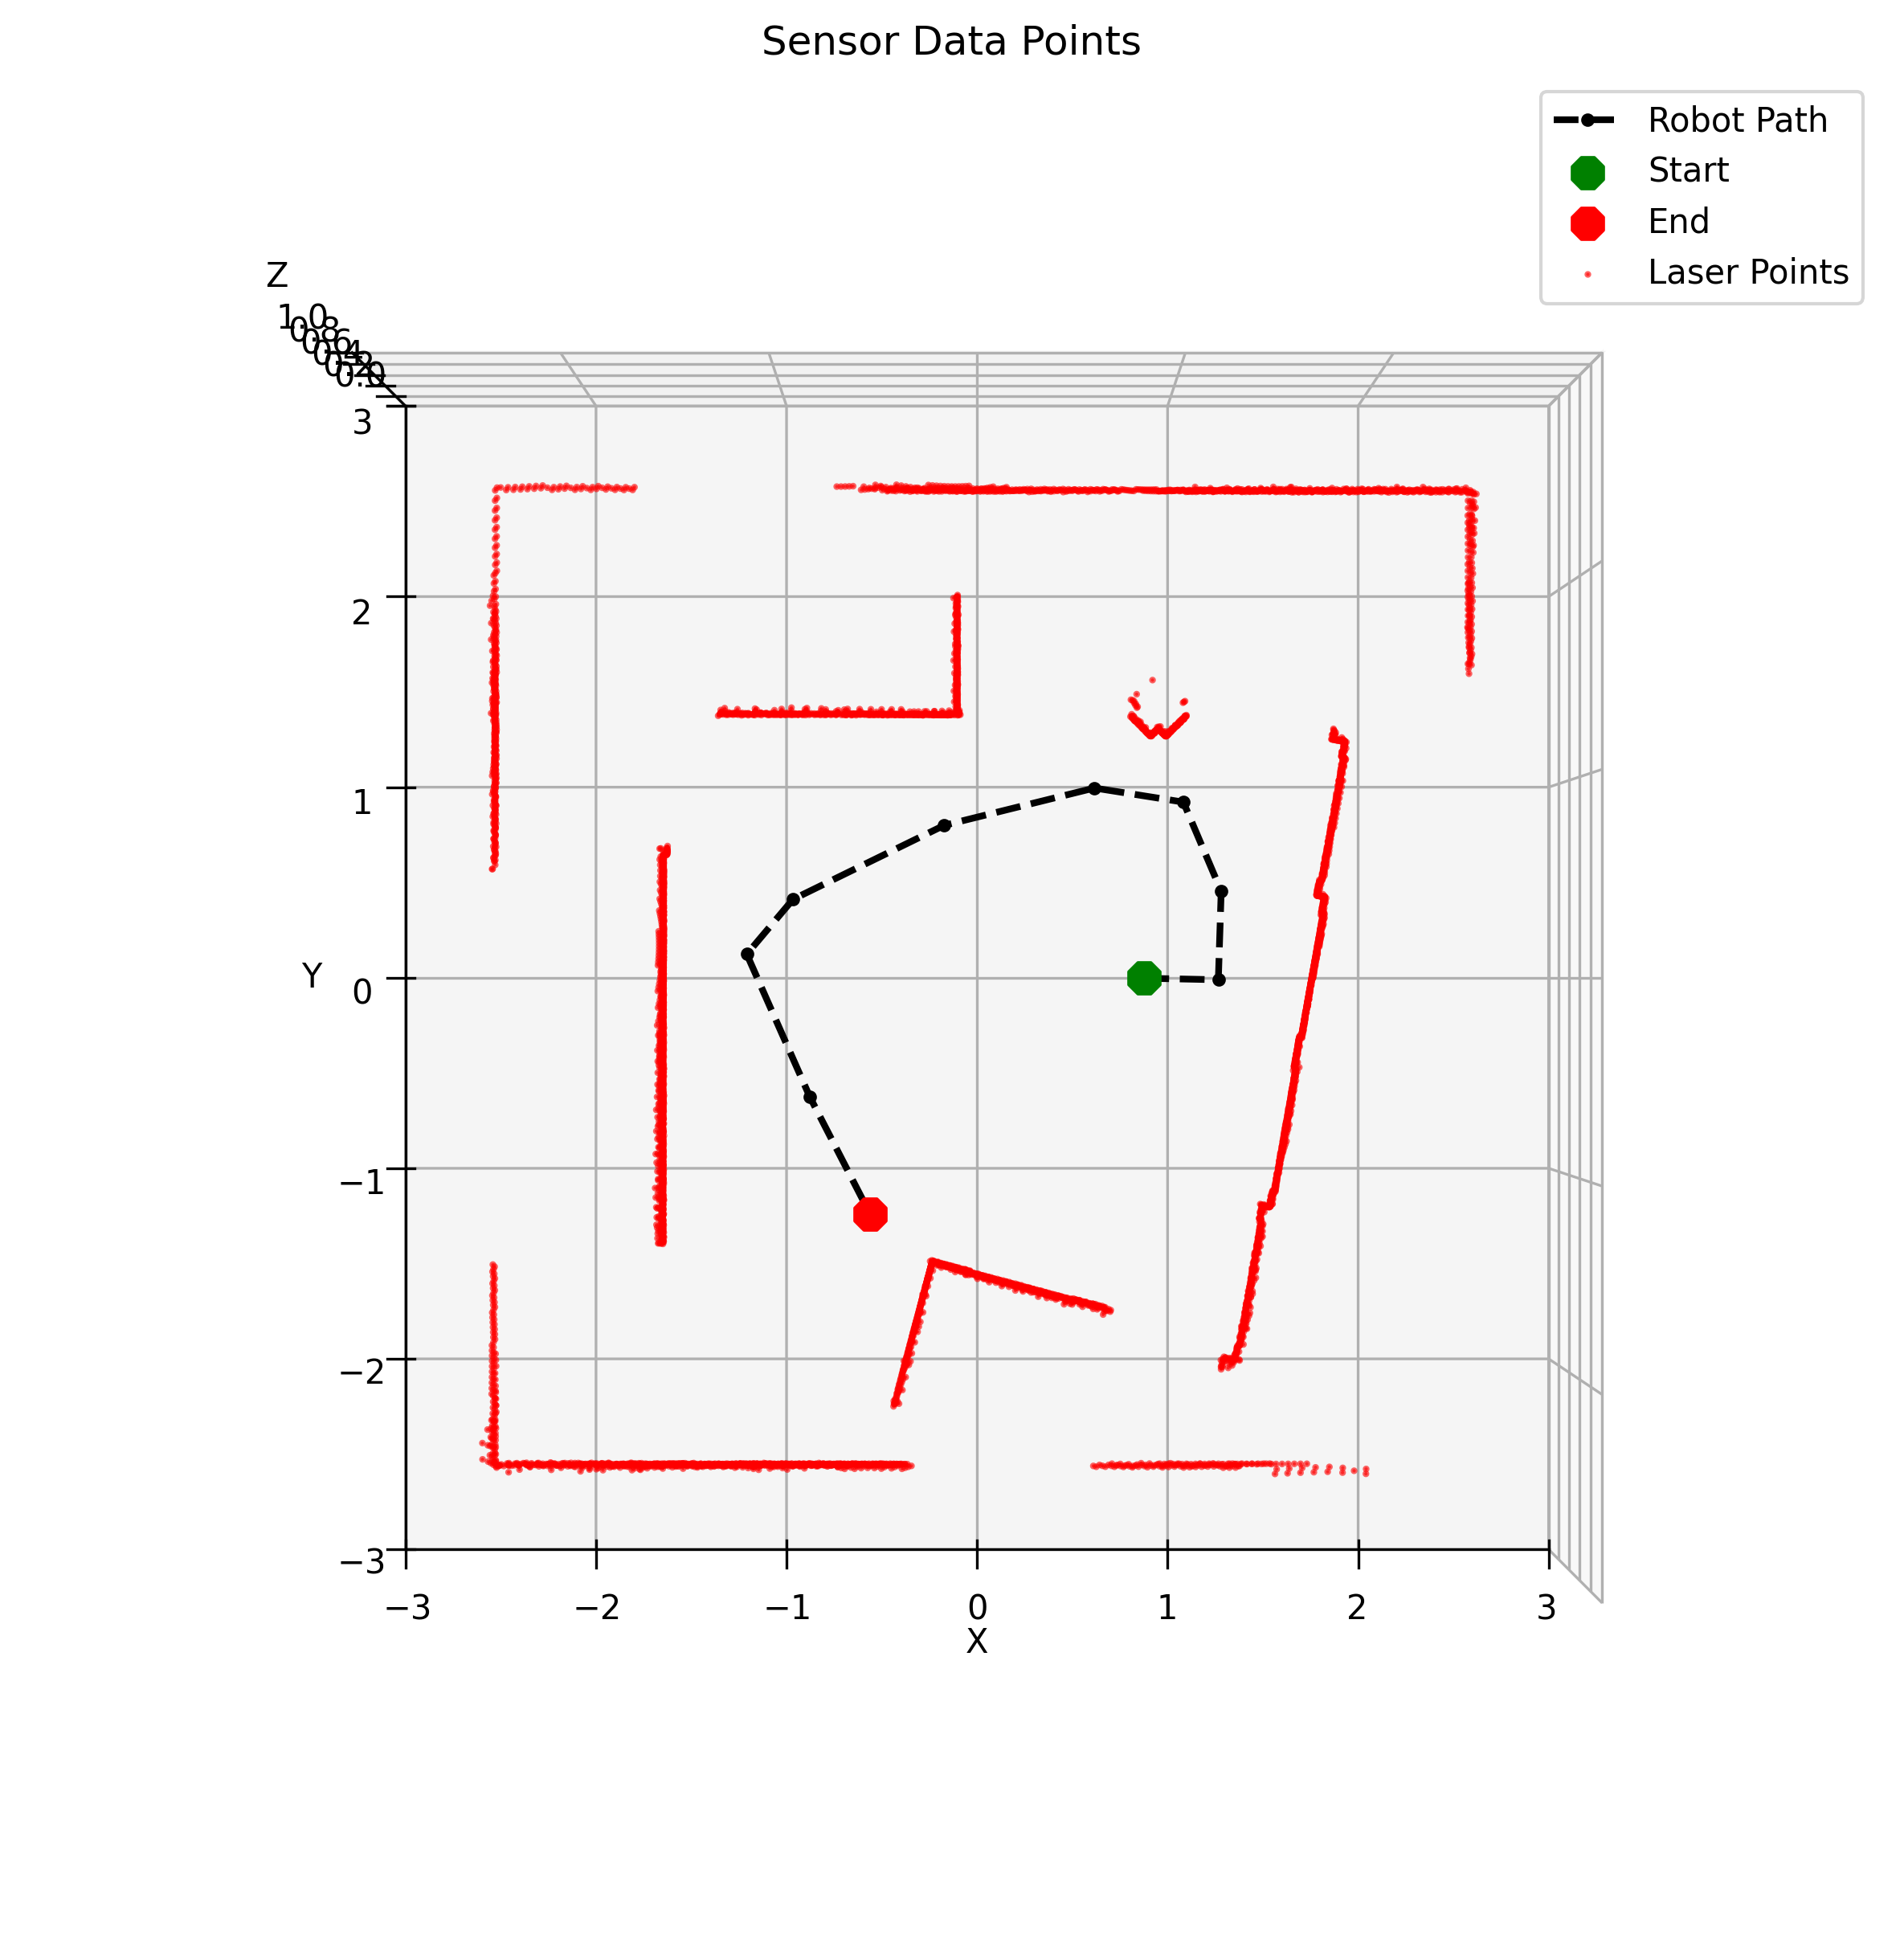
\includegraphics[width=\linewidth]{plots/q6.png}
  \caption{Trajetória do robô (linha tracejada) e todas as leituras do laser acumuladas em \(W\).}
\end{figure}

% ============================
\section*{Conclusão}
Este trabalho consolidou o uso de matrizes de transformação homogênea e a composição de transformações entre frames para robótica móvel. A integração com o CoppeliaSim e a RemoteAPI exigiu cuidado na conversão entre diferentes formatos de pose (HTM \(4\times4\), representações \(3\times4\) e quaternion). O uso de \emph{stepping} foi fundamental para garantir a consistência das leituras do laser ao longo do tempo, evitando erros por transformação com poses incorretas durante o movimento do robô.

O principal desafio identificado consistiu em assegurar a correção do último gráfico. Observou-se que, quando a simulação era executada de forma contínua, o processo de coleta dos dados do sensor Hokuyo demandava um tempo \textit{T} geralmente muito superior ao passo de simulação \textit{dt}. Como consequência, o robô permanecia em movimento durante esse intervalo, o que comprometia a consistência dos dados. Em situações em que tal aspecto não era considerado, o resultado gráfico apresentava distorções significativas: parte dos pontos era coletada enquanto o robô se deslocava, porém todos eram transformados assumindo a mesma pose, ocasionando um desvio perceptível no gráfico final. Para mitigar esse problema, implementou-se a execução passo a passo da simulação. 

Nesse procedimento, a simulação era interrompida imediatamente antes da coleta, garantindo que todos os pontos fossem registrados em uma única configuração do robô. Após a conclusão da coleta, a simulação era retomada com a execução de um novo passo (\texttt{step()}). Isso fez com que o gráfico final fosse plotado de maneira correta.

\end{document}
